% Macros to fixup import locations
\newcommand{\DrownPaper}{papers/drown/paper}
\newcommand{\DrownFigures}{papers/drown/figures}

% include command definitions
% !TEX root = ../../../proposal.tex
% General definitions and terms
% \newcommand{\PKCS}{PKCS\#1 v1.5\xspace}
% \newcommand{\PKCSconform}{\PKCS\ conformant\xspace}
% \newcommand{\sslconform}{SSLv2 conformant\xspace}
% \newcommand{\tlsconform}{TLS conformant\xspace}
% \newcommand{\Enc}{\mathsf{Enc}}
% \newcommand{\Dec}{\mathsf{Dec}}
% \newcommand{\OBleichenbacher}{\mathcal{O}_\textsf{BB}}
% \newcommand{\Oracle}{\mathcal{O}}
% \newcommand{\pms}{premaster secret\xspace}
% \newcommand{\ssltwo}{SSLv2\xspace}
% \newcommand{\sslthree}{SSLv3\xspace}
% \newcommand{\hashcomputation}{hash computation\xspace} % todo rename???

% hex helpers
\newcommand{\hexspace}{\hspace{0.06cm}}
\newcommand{\hexhelp}[2]{#1\hexspace#2}
\newcommand{\hexhelpb}[4]{\hexhelp{#1}{#2}\hexspace\hexhelp{#3}{#4}}
\newcommand{\hex}[1]{{\tt 0x#1}}
\newcommand{\hexb}[2]{{\tt 0x\hexhelp{#1}{#2}}}
\newcommand{\hexc}[3]{{\tt 0x\hexhelp{#1}{#2}\hexspace#3}}
\newcommand{\hexd}[4]{{\tt 0x\hexhelp{#1}{#2}\hexspace\hexhelp{#3}{#4}}}
\newcommand{\hexh}[8]{{\tt 0x\hexhelpb{#1}{#2}{#3}{#4}\hexspace \hexhelpb{#5}{#6}{#7}{#8}}}

% feel free to rename oracles 
\newcommand{\OracleSSL}{\mathcal{O}_\textsf{SSLv2}}
\newcommand{\OracleSSLexp}{\mathcal{O}_\textsf{SSLv2-export}}
\newcommand{\OracleSSLclear}{\mathcal{O}_\textsf{SSLv2-extra-clear}}
\newcommand{\OracleSSLleaky}{\mathcal{O}_\textsf{SSLv2-export-leaky}}

\newcommand{\tOracleSSLexp}{SSLv2 export oracle\xspace}
\newcommand{\tOracleSSLclear}{Extra Clear oracle\xspace}
\newcommand{\tOracleSSLleaky}{Leaky Export oracle\xspace}

\newcommand{\pos}[1]{{[#1]}}


% Keep extra detail for the extended version
\newif\ifext\extfalse
\newif\ifdraft\draftfalse
\newif\ifblind\blindtrue
\newif\ifsubmit\submitfalse

\draftfalse
\blindfalse
%\exttrue

% \ns (``number space''): Insert space equivalent to a number, to avoid needing leading zeros to align numbers in tables; first argument specifies a multiplier (AH 4/2016)
%     Example: 100%\\ \ns 50% \\ \ns[2] 1%
\newlength{\nswidth}\newcommand{\ns}[1][1]{\settowidth{\nswidth}{0}\hspace{#1\nswidth}}

\newcommand{\tabDrownAll}{
  \begin{table*}[t]
  \centering\small
  \begin{tabularx}{\textwidth}{Xrrrrrrr} 
  \toprule
  & & \multicolumn{3}{c}{\it Any certificate} & \multicolumn{3}{c}{\it Trusted certificates} \\
  \cmidrule(lr){3-5} \cmidrule(lr){6-8}
  \textbf{Protocol} & \textbf{Port} & \textbf{SSL/TLS}  & \twolinecell{\bf \ssltwo \\\bf support}        & \twolinecell{\bf Vulnerable\\\bf key} & \textbf{SSL/TLS} & \twolinecell{\bf \ssltwo\\\bf support} &  \twolinecell{\bf Vulnerable \\\bf key} \\
  \midrule
  SMTP     & 25  & 3,357\,K &   936\,K (28\%)  & 1,666\,K (50\%)  &  1,083\,K  &   190\,K (18\%) & 686\,K (63\%)   \\
  POP3     & 110 & 4,193\,K &   404\,K (10\%)  & 1,764\,K (42\%)  &  1,787\,K  &   230\,K (13\%) & 1,031\,K (58\%) \\
  IMAP     & 143 & 4,202\,K &   473\,K (11\%)  & 1,759\,K (42\%)  &  1,781\,K  &   223\,K (13\%) & 1,022\,K (57\%) \\
  HTTPS    & 443 & 34,727\,K& 5,975\,K (17\%)  & 11,444\,K (33\%) &  17,490\,K & 1,749\,K (10\%) & 3,931\,K (22\%) \\
  SMTPS    & 465 & 3,596\,K &   291\,K \ns (8\%)   & 1,439\,K (40\%)  &  1,641\,K  &     40\,K \ns (2\%) & 949\,K (58\%)   \\
  SMTP     & 587 & 3,507\,K &   423\,K (12\%)  & 1,464\,K (42\%)  &  1,657\,K  &    133\,K \ns (8\%) & 986\,K (59\%)   \\
  IMAPS    & 993 & 4,315\,K &   853\,K (20\%)  & 1,835\,K (43\%)  &  1,909\,K  &   260\,K (14\%) & 1,119\,K (59\%) \\
  POP3S    & 995 & 4,322\,K &   884\,K (20\%)  & 1,919\,K (44\%)  &  1,974\,K  &   304\,K (15\%) & 1,191\,K (60\%) \\
  \midrule
  (Alexa~Top~1M) & 443 & 611\,K   & 82\,K (13\%)     & 152\,K (25\%)  & 456\,K     & 38\,K \ns (8\%)     & 109\,K (24\%)   \\
%% \ifext
%% \else
%%   \midrule
%%   \bf Special DROWN:\smallskip\\
%%   HTTPS & 443 & 34,727\,K  & 4,029\,K (12\%) & 9,089\,K (26\%) & 17,490\,K & 2,523\,K (14\%) & 3,793\,K (22\%) \\
%%     (Alexa~1M) & 443 & 611\,K & 22\,K (4\%)  & 52\,K (9\%)     & 456\,K & 33\,K (7\%)     & 85\,K (19\%)    \\
%% \fi
  \bottomrule
   \end{tabularx}
   \caption{\textbf{Hosts vulnerable to general DROWN\@.} We performed Internet-wide scans to measure the number of hosts supporting \ssltwo on several different protocols.  A host is vulnerable to DROWN if its public key is exposed anywhere via \ssltwo.  Overall vulnerability to DROWN is much larger than support for \ssltwo due to widespread reuse of keys.}
   \label{table:general}
  \end{table*}
}

\newcommand{\tabSpecialAll}{
\begin{table*}[t]
  \centering\small
  \begin{tabularx}{\textwidth}{Xrrrrrrr}
    \toprule
    & & \multicolumn{3}{c}{\it Any certificate} & \multicolumn{3}{c}{\it Trusted certificates} \\
    \cmidrule(lr){3-5} \cmidrule(lr){6-8}
    \textbf{Protocol} & \textbf{Port} & \multicolumn{1}{c}{\bf SSL/TLS} & \twolinecell{\bf Special DROWN\\\bf oracles} & \twolinecell{\bf Vulnerable\\\bf key} & \multicolumn{1}{c}{\bf SSL/TLS} & \twolinecell{\bf Vulnerable\\\bf key} & \twolinecell{\bf Vulnerable\\\bf name} \\
    \midrule
    SMTP  & 25  & 3,357\,K   & 855\,K (25\%)   & 896\,K (27\%)   & 1,083\,K  & 305\,K (28\%)   & 398\,K (37\%)   \\
    POP3  & 110 & 4,193\,K   & 397\,K \ns (9\%)    & 946\,K (23\%)   & 1,787\,K  & 485\,K (27\%)   & 674\,K (38\%)   \\
    IMAP  & 143 & 4,202\,K   & 457\,K (11\%)   & 969\,K (23\%)   & 1,781\,K  & 498\,K (30\%)   & 690\,K (39\%)   \\
    HTTPS & 443 & 34,727\,K  & 4,029\,K (12\%) & 9,089\,K (26\%) & 17,490\,K & 2,523\,K (14\%) & 3,793\,K (22\%) \\
    SMTPS & 465 & 3,596\,K   & 334\,K \ns (9\%)    & 765\,K (21\%)   & 1,641\,K  & 430\,K (26\%)   & 630\,K (38\%)   \\
    SMTP  & 587 & 3,507\,K   & 345\,K (10\%)   & 792\,K (23\%)   & 1,657\,K  & 482\,K (29\%)   & 667\,K (40\%)   \\
    IMAPS & 993 & 4,315\,K   & 892\,K (21\%)   & 1,073\,K (25\%) & 1,909\,K  & 602\,K (32\%)   & 792\,K (42\%)   \\
    POP3S & 995 & 4,322\,K   & 897\,K (21\%)   & 1,108\,K (26\%) & 1,974\,K  & 641\,K (32\%)   & 835\,K (42\%)   \\
    \midrule
    (Alexa~Top~1M) & 443 & 611\,K & 22\,K \ns (4\%)  & 52\,K \ns (9\%)     & 456\,K    & 33\,K \ns (7\%)     & 85\,K (19\%)    \\
    \bottomrule
  \end{tabularx}
   \caption{\textbf{Hosts vulnerable to special DROWN.} A server is vulnerable to special DROWN if its key is exposed by a host with the CVE-2016-0703 bug. Since the attack is fast enough to enable man-in-the-middle attacks, a server is also vulnerable (to impersonation) if any name in its certificate is found in any trusted certificate with an exposed key.}
   \label{table:special}
\end{table*}
}



%\section*{Abstract}
% !TEX root = proposal.tex
\abstract{
Cryptography is a key component of the security of the Internet.
Unfortunately, the process of using cryptography to secure the Internet is
fraught with failure. Cryptography is often fragile, as a single mistake can
have devastating consequences on security, and this fragility is further
complicated by the diverse and distributed nature of the Internet. This
dissertation shows how to use empirical methods in the form of Internet-wide
scanning to study how cryptography is deployed on the Internet, and shows
this methodology can discover vulnerabilities and gain insights into fragile
cryptographic ecosystems that are not possible without an empirical approach.
I introduce improvements to ZMap, the fast Internet-wide scanner, that allow
it to fully utilize a 10\,GigE connection, and then use Internet-wide
scanning to measure cryptography on the Internet.

First, I study how Diffie-Hellman is deployed, and show that implementations
are fragile and not resiliant to small subgroup attacks. Next, I measure the
prevalence of ``export-grade'' cryptography. Although regulations limiting
the strength of cryptography that could be exported from the United States
were lifted in 1999, Internet-wide scanning shows that support for various
forms of export cryptography remains widespread. I show how purposefully
weakening TLS to comply with these export regulations led to the FREAK,
Logjam, and DROWN vulnerabilities, each of which exploits obsolete
export-grade cryptography to attack modern clients. I conclude by discussing
how empirical cryptography improved protocol design, and I present further
opportunities for empirical research in cryptography.

\paragraph{Thesis Statement.} Large-scale empirical methods allow us to
observe fragility in how cryptography is being used on the Internet, identify
new vulnerabilities, and better secure the Internet in the future.
}


\section{Introduction}
% !TEX root = ../proposal.tex

Cryptography is mathematical science. Cryptography research is often formal,
and concerned with proving the correctness of primitives and
protocols, given some set of assumptions. Cryptography is one of the only
components of security that can be provably secure. As such, cryptography is
often considered to be one of the strongest components of security.

Yet historically, cryptography has been one of the most \textit{fragile}
aspects of security. This fragility is often not because the underlying math
was incorrect, or because the fundamental cryptographic primitives were
insecure, but because a single mistake in the implementation, configuration,
or protocol can have catastrophic effects on security. Security is lost in
translation between the cryptographers and protocol designers, and between
protocol designers and implementers. The process of going from paper to
program, or from proof-of-concept to production, introduces mistakes and
misunderstandings and reveals incorrect assumptions. This leads to
cryptographic failures and insecurity.

%To address this, the cryptographic research community is beginning to
%introduce and study new concepts such as misuse-resistant cryptography, and
%simplified cryptographic APIs. Unfortunately, the state of the art in
%cryptography engineering remains considerably behind the state of art in
%research.

Cryptography is a key component in the security of the Internet.
Unfortunately, the fragile nature of cryptography can be compounded by the
large-scale, distributed, and diverse nature of the Internet. Any protocol
can have many implementations, each of which may implement different subsets
of the protocol, or support different configurations. Many protocols are
designed for ``cryptographic agility'', and so identical implementations may
support different sets of underlying algorithms. Devices that support modern
cryptography may also support decades-old broken cryptography. This leads to
an Internet of fragile cryptographic ecosystems, consisting of diverse sets
of clients and servers \todo{define this more}.

%To better use cryptography to secure the Internet, we must first
%understand how cryptography is being used on the Internet. Examining CVE databases
%and trawling through cryptographic code provides one lens into real-world
%deployments of cryptography, but does not necessarily reflect the state of
%the Internet.

To better use cryptography to secure the Internet, we need to understand what
types of cryptography are being used, and where mistakes are being made. We
must understand which cryptographic ecosystems are fragile, and which are
resiliant. Large-scale empirical methods allow us to observe fragility in
how cryptography is being used on the Internet, identify new vulnerabilites,
and better secure the Internet in the future.

In this dissertation, I show how empirical measurements collected using
Internet-wide scanning provides insight into how cryptography is used to
secure the Internet. First, I show contributions made to the field of
Internet measurement field itself via improved Internet-wide scanning.
Second, I measure the Internet's resiliancy to small subgroup attacks in
finite-field Diffie-Hellman. Third, I use empirical methods to show how
1990s-era export-grade encryption harmed the security of the Internet for two
decades.

\section{Techniques for Measuring Internet Cryptography}

Internet-wide scanning is a fundmental technique used for empirical study of
cryptography. Large-scale, horizontal port scanners such as
ZMap~\cite{zmap-2013} drastically reduce the barrier to entry to leveraging
network scan data at Internet scale, however port scanning alone is not a
complete solution. Using Internet-wide scanning to measure cryptography is a
three step process:
\begin{enumerate}
  \item \textbf{Identify Hosts.}
    There are $\sim$4B possible IPv4 addresses, however only a subset are
    listening on any given L4 port. A single scan by ZMap or another
    large-scale, asynchronous L3/L4 scanner identifies which hosts have an
    input port open. For example, only $\sim$50M hosts respond on TCP port 443
    (HTTPS).
  \item \textbf{Measure Hosts.}
    ZMap provides no application-layer information about a host. Furthermore,
    hosts that respond on a standard port for some application-layer protocol
    might not actually be configured to speak that protocol. For example,
    only $\sim$38M of the $\sim$50M hosts with TCP port 443 open are TLS
    servers. To collect cryptographic data, an application-layer scanner such
    as ZGrab~\cite{zgrab-github} must connect to all hosts found by ZMap and
    attempt a protocol handshake that records the cryptographic state used
    for the connection.
  \item \textbf{Answer Questions.}
    As is the case in any empirical science, the measurement data is analyzed
    to answer questions such as ``What percentage of TLS servers support
    512-bit Diffie-Hellman?''. Tools such as Censys~\cite{censys} allow
    researchers to ask questions about Internet-wide scan data much faster
    and easier than by trawling through results from individual scans, each
    of which can generate terabytes of data.
\end{enumerate}

With current technology, Internet-wide scanning is useful for creating an
aggregate understanding of the Internet over time. However, it is not yet
able to provide a global understanding of \textit{individual} hosts and
networks. I first discuss contributions to Internet-wide scanning that
provide a foundation to build a more accurate and complete picture of the
Internet in \S\ref{chapter:zippier}. I show improvements to the ZMap scanner
which enable it to operate at a full 10Gbps line
rate~\cite{zippier-zmap-2014}. While ZMap enabled the use of Internet-wide
scanning accessible as a measurement method, this work moves towards enabling
hourly or real-time measurement of the cryptographic behavior of all
Internet-connected systems.

When originally introduced, ZMap was capable of saturating a 1Gbps uplink from
a single host, enabling an Internet-wide TCP SYN scan of IPv4 to be performed
in forty-five minutes. However, when used with a 10Gbps network interface, ZMap
reached barely above the 1Gbps mark. The required thread synchronization during
address generation restricted the performance benefit of threading, and limited
the ability to leverage multi-core systems. Furthermore, the copy from user
space to kernel memory when sending a packet limited total throughput. Scanning
a 10Gbps requires sending nearly 15 million packets per second continuously,
which allows for only 200 cycles per packet on a 3 GHz system.

I introduced performance improvements to address both of these constraints, and
enable ZMap to fully utilize a 10Gbps network link, bringing the total time for
a TCP SYN scan of IPv4 to under five minutes from a single host. While
Internet-measurement is often used to provide coarse-grain understanding of the
shape of the Internet as a whole, improvements in measurement-collection begin
to move the field towards being able to continuously understand the behavior of
individual hosts, but at global scale.

\section{Measuring Diffie-Hellman}

There is a knowledge gap between implementers and researchers. Cryptographers
can be aware of attacks for decades, but this doesn't necessarily translate
into concrete steps that implementers can take to avoid vulnerability. A
specific example of this is prime-field based Diffie-Hellman key exchange, in
which implementation and hosts often use groups which unnecessarily open up
the likelihood of small-subgroup confinement and key recovery
attacks~\cite{subgroup-2017}. I used empirical techniques to provide insight
into the Diffie-Hellman group selection at Internet-scale, showing that while
a common recommendation is that $p$ should be a ``safe'' prime such that $p =
2q+1$ for some prime $q$, many implementations instead use non-safe ``DSA''
parameters with potentially unsafe subgroups of order $q$. Several standards,
including NIST~SP~800-56A~\cite{sp800} and RFC~5114~\cite{rfc5114}, advocate
the use of these parameters for Diffie-Hellman key exchange, and while it is
possible to use such parameters securely, additional validation checks are
necessary to prevent small-subgroup attacks.

We measured the prevalence of these parameter choices in the wild for HTTPS,
POP3S, SMTP with STARTTLS, SSH, IKEv1, and IKEv2, finding millions of hosts
using DSA and other non-``safe'' primes for Diffie-Hellman key exchange, many
of them in combination with potentially vulnerable behaviors. Beyond simply
using DSA primes, small subgroup attacks require a number of complex, special
conditions to go wrong in order to be feasible, described in
\S\ref{chapter:subgroup}. While seems unlikely that any implementation would
satisfy enough of these requirements to be vulnerable to an attack, it also
seemed unlikely that implementations would use non-safe primes for key
exchange in the first place. Empirical methods did not reveal an
Internet-wide vulnerability, but rather an Internet-wide case of accidental
complexity and fragility. Given the amount of complexity exposed by the
underlying cryptographic APIs for Diffie-Hellman, it is remarkable that any
implementation was safe. Understanding the root causes of this complexity and
confusion, and understanding how it manifests on the Internet, enables better
protocol design in the future.

\section{Measuring Export Cryptography}

%Discrete-log and factoring based attacks are generally considered out of reach
%of attackers.  However, informing such attacks with measurement data allows for
%cost-effective attacks that leverage a single, expensive pre-computation to
%cheaply attack TLS connections. Furthermore, when combined with broad support
%for cryptography that was assumed to be “dead”, these attacks become even
%cheaper.

%\paragraph{Export Cryptography}

The Department of State regulated cryptography in the United States during
the 1990s. Cryptography was covered by the Internation Traffic in Arms
Regulations (ITAR), which broadly limited the ability for US persons to
``export'' cryptography. Beginning in 1995, these regulations were challenged
in court by Daniel J. Bernstein, who was attempting to publish the
``Snuffle'' cryptosystem. The regulations were moved in 1996 from ITAR to the
Export Administration Regulations (EAR), under the control of the Department
of Commerce~\cite{djb-case-status}. Under EAR, ``exported'' cryptography was
limited to 40-bits of security for symmetric ciphers, and 512-bits for
security for public-key cryptography. Authentication strength (\eg MAC
length), was not regulated~\cite{ear-2001-cat-5}. Despite these limitations,
there were major advances in secure channel protocol development during this time.
\ssltwo was designed and deprecated~\cite{sslv2} in 1995. SSLv3 was created and
standardized~\cite{rfc6101} by 1998, and subsequently renamed to TLS and
moved into the purview of the IETF in 1999~\cite{rfc2246}. All three of these
protocol versions contained compliance mechanisms for the export regulations,
where the protocol was capable of negotiating the use of short
``export-grade'' parameters instead of ``modern'' cryptography.

Following further litigation in \textit{Bernstein vs United States}, the key
length limitations from the export regulations were removed in 1999, and
future versions of TLS deprecated the process for using ``export-grade''
cryptography.

\subsection{Attacks on RSA}

\todo{freak}

\todo{freak measurements}

\subsection{Attacks on Diffie-Hellman}

Diffie-Hellman key exchange is one of the most common public-key
cryptographic methods in use in the Internet. In finite field Diffie-Hellman,
Alice and Bob agree on a large prime $p$ and an integer $g$ modulo $p$. Alice
chooses a secret integer $x_a$ and transmits a public value $g^{x_a} \bmod
p$; Bob chooses a secret integer $x_b$ and transmits his public value
$g^{x_b} \bmod p$. Both Alice and Bob can reconstruct a shared secret $g^{x_a
x_b} \bmod p$, but the best known way for a passive eavesdropper to
reconstruct this secret is to compute the discrete log of either Alice or
Bob's public value. Specifically, given $g$, $p$, and $g^x \bmod p$, an
attacker must calculate $x$.

We uncovered several weaknesses in how finite-field Diffie-Hellman key
exchange was deployed, which drastically affected the cost of decrypting
large amounts of TLS traffic. The algorithmic complexity of calculating
discrete log is exponential, but the bulk of this computation is dependent
solely on $p$, not the individual secrets $a$ and $b$ chosen by each party.
If many hosts use the same groups, then the precomputation cost may be
amortized across all the connections across these hosts, rather than
requiring core-centuries per observed key exchange. This raise an obvious
empirical question: do many hosts share the same set of Diffie-Hellman
parameters, and what is the strength of the parameters?

The TLS protocol contains ``export-grade'' Diffie-Hellman ciphers which use
short 512-bit groups. We show that there is a protocol vulnerability in TLS,
named Logjam, which allows an attacker who can calculate 512-bit discrete logs
to downgrade connections to export-grade Diffie-Hellman ciphers, and decrypt
them. If a TLS session were to use 512-bit Diffie-Hellman, it may first appear
that individual connections could be broken in 60,000 core-hours, or 120 hours
in parallel on commodity hardware. While this is certainly insecure, at first
glance it would appear these connections have a small amount forward secrecy,
by virtue of using ephemeral Diffie-Hellman key, e.g. each connection would
require another 120 hours to be decrypted. This slow process would prohibit
active attacks and limit the risk to passive decryption after the fact. This
again falls prey to precomputation: if many hosts were to support the same weak
parameters, then the computation could be amortized, and individual connections
could be broken in real-time, enabling active attacks. In fact, shared sets of
parameters is what enables the downgrade. In this case, empirical measurement
showed that 80\% of vulnerable hosts used the same set of parameters, moving
this attack from the theoretical to the practical. While recently there has
been a trend towards elliptic curve cryptography, prime-field based
Diffie-Hellman remained common in TLS until 2016, when both Firefox and Chrome
removed it from their default cipher suites as a result of our work.

\subsection{Cross-Protocol Attacks}

Reusing TLS keys across multiple protocols, such as HTTPS, SMTP, and IMAP,
leads to an increased attack surface. Empirical methods allow us to understand
the attack surface increase from key reuse. Furthermore, specific
vulnerabilities in the TLS protocol and older implementations can be utilized
in a cross-protocol context to attack users of a web service without explicitly
compromising the private key. This is best shown by the DROWN vulnerability, in
which the mere existence of an \ssltwo host that shared a key with a TLS host
enabled decryption of otherwise secure TLS connections using modern
cryptography.

The DROWN attack further exploited export-grade cryptography with an additional
novel insight: Bleichenbacher oracles need not be present in the target
protocol under attack, so long as the key is shared between the two protocols.
Specifically, DROWN shows how to use protocol vulnerabilities in \ssltwo to
attack TLS 1.2. The \ssltwo protocol includes support export symmetric ciphers
which are seeded via only five bytes of key material encrypted using RSA \PKCS.
The \ssltwo protocol also requires the server to send data to the client that is
derived from the shared secret, without first verifying that the client has
possession of the secret. When combined with the malleability of RSA,
culminates in a Bleichenbacher oracle that can be used to attack TLS 1.2

Beyond DROWN, the TLS protocol has a fundamentally cross-protocol attack
surface. X.509 certificates are not bound to any particular protocol or port.
Furthermore, even if distinct services, such as mail and web servers, use
different keys, so long as they share any name on the certificate, the
transport-layer security of all connections to that name are limited to the
security of the weakest TLS implementation or configuration. Even traditionally
web-based padding oracle attacks, such as POODLE, or the AES-NI padding-oracle
in OpenSSL, non-web servers can be exploited by active attackers targeting web
users. The attacker can rewrite the TCP connection to an alternative port, and
fill-in any pre-handshake protocol dialogue (e.g. by sending an EHLO or
STARTTLS command in SMTP). Ignoring vulnerabilities in TLS itself, an unpatched
piece of software with a known RCE using the same key as a well-configured and
up to date web server places web clients, should the key be stolen via
traditional software exploitation. We can place an upper bound on the increased
attack surface, by measuring key and name reuse across TLS in different
application-layer protocols on different ports.

\subsection{Weaknesses from Export Cryptography}

As shown by Freak, Logjam, and DROWN, the security of TLS and export
cryptography are fundamentally linked. Export cryptography is a unique
constraint with a fundamentally dangerous goal: weaken cryptography, without
weakening cryptography. Internet measurement techniques show us that the export
regulations weakened protocol design to the point where the regulations are
directly harmful to the security of the Internet today. These empirical
techniques show that these attacks are not theoretical, leveraging protocols
that have long-since disappeared, but instead are a dark side of backwards
compatibility, harming real users today. Although the regulations went out of
effect by 1999, the cryptography remains. At their respective times of
disclosure, 36.7\% of IPv4 HTTPS hosts were vulnerable to FREAK, 4.9\% were
vulnerable to Logjam, and 26\% were vulnerable to DROWN. All forms of export
cryptography have been broken: export RSA key exchange was broken by FREAK,
export Diffie-Hellman key exchange was broken by Logjam, and export symmetric
ciphers were broken by DROWN. In all cases, empirical research enabled the full
understanding of the effects and impacts of these issues.

% CONCLUSION THOUGHTS
% 
% ENGINERING?
% 
% Applying empirical measurement techniques accurately requires careful
% application of the scientific method and experiment design. However, the field
% of Internet-measurement has strong engineering underpinnings which are often
% overlooked. ZMap now provides efficient transport-layer scanning, but
% application-layer scanning has not yet reached the same efficiency as ZMap.
% Tooling such as ZGrab helps fill in some of these gaps, but is not yet
% transformative. Similarly, simply studying HTTPS at scale creates unique
% engineering constraints, such as how to batch parse and validate X.509
% certificates.



\section{Background}
%\subsection{Bleichenbacher's Attack.}
%One of the most important attacks in the TLS history is the million's message attack, published by Daniel Bleichenbacher at Crypto 1998~\cite{Bleichenbacher}. The attack targets the RSA \PKCS encryption scheme, which is used in the TLS protocol to encrypt a so called \pms. The \pms a 48 byte value sent by the client to the server, encrypted using server's public key. Based on the \pms, both peers can derive \textit{all} keys needed for secure communication.
%
%Essentially, Bleichenbacher's attack is an adaptive chosen-ciphertext attack or, more commonly known, a padding oracle attack. The attack assumes existence of an oracle that responds with "valid" or "invalid" according to the \PKCS validity of the decrypted message. The attacker exploits such an oracle as follows. It starts the attack with an RSA ciphertext (containing an encrypted \pms), which he obtained for example by observing the traffic between the client and the server. The attacker then modifies this ciphertext, sends it to the server, and observes the ciphertext validity. With each valid ciphertext, the attacker learns several plaintext bits. At the end, by sending several thousands of messages the attacker can decrypt the whole \pms, and thereby decrypt a TLS session.

In the following, $a||b$ denotes concatenation of strings $a$ and
$b$. $a{[i]}$ references the $i$-th byte in $a$.
$(N,e)$ denotes an RSA public key, where $N$ has byte-length
$\ell_m$ ($|N|=\ell_m$) and $e$ is the public exponent. The corresponding
secret exponent is $d = 1/e \bmod \phi(N)$.

\subsection{\PKCS encryption padding}
\label{sec:PKCSdescr}

Our attacks rely on the structure of RSA \PKCS padding.  Although RSA PKCS\#1 v2.0
implements OAEP, SSL/TLS still uses \PKCS.
The \PKCS encryption padding scheme~\cite{rfc2313}
randomizes encryptions by prepending a random padding string $PS$
to a message $k$ (here, a symmetric session key) before
RSA encryption:

\begin{enumerate} 
	\item The plaintext message is $k$, $\ell_k = |k|$. The encrypter generates a random byte
	string $PS$, where $|PS| \geq 8$, $|PS|=\ell_m-3-\ell_k$, and $\hex{00} \not \in \{PS{[1]}, \ldots,PS{[|PS|]}\}$. 
	\item The encryption block is $m = 00||02||PS||00||k$. 
	\item The ciphertext is computed as $c = m^e \bmod N$. 
\end{enumerate} 

To decrypt such a ciphertext, the decrypter first computes $m = c^d
\bmod N$.  Then it checks whether the decrypted message $m$ is
correctly formatted as a \PKCS-encoded message. We say that the
ciphertext $c$ and the decrypted message bytes $m{[1]} || m{[2]} || ... ||
m{[\ell_m]}$ are \PKCSconform if:
\begin{equation*} 
	\begin{split} 
		m{[1]}||m{[2]} \text{ } = &\text{ } \hex{00} || \hex{02}\\
		\hex{00} \text{ } \not \in &\text{ } \{m{[3]}, \ldots,m{[10]}\}\\ 
	\end{split}
\end{equation*} 
If this condition holds, the decrypter searches for the first value
$i>10$ such that $m{[i]}=0x00$. Then, it extracts $k =
m{[i+1]}||\ldots||m{[\ell_m]}$. Otherwise, the ciphertext is rejected.

In SSLv3 and TLS, RSA \PKCS is used to encapsulate the
\pms exchanged during the
handshake~\cite{rfc5246}. Thus, $k$ is interpreted as the
\pms.  In SSLv2, RSA \PKCS is used for
encapsulation of an equivalent key denoted the \texttt{master\_key}.


\subsection{SSL and TLS}
The first incarnation of the TLS protocol was the SSL (Secure Socket
Layer) protocol, which was designed by Netscape in the 90s. The first two
versions of SSL were immediately found to be vulnerable to trivial
attacks~\cite{ProhibitingSSLv2,WagnerSchneier:SSLAnalysis:96} which 
were fixed in SSLv3~\cite{SSLv3}.  Later versions of
the standard were renamed TLS, and share a similar structure to SSLv3.
The current version of the protocol is TLS 1.2; TLS 1.3 is currently
under development.

An SSL/TLS protocol flow consists of two phases: handshake and
application data exchange. In the first phase, the communicating
parties agree on cryptographic algorithms and establish shared
keys. In the second phase, these keys are used to protect the
confidentiality and authenticity of the transmitted application data.

The handshake protocol was fundamentally redesigned in the \sslthree
version. This new handshake protocol was then used in later TLS
versions up to TLS 1.2. In the following, we describe the RSA-based
handshake protocols used in TLS and \ssltwo, and highlight their
differences.

%\paragraph{Cipher Suites.}
%The SSL/TLS protocol flow uses different cryptographic algorithms for data encryption, signature computation, or HMAC generation. A set of cryptographic algorithms used during a protocol flow is summarized in a cipher suite. For example, a \texttt{TLS\_RSA\_WITH\_AES\_128\_CBC\_SHA} cipher suite denotes that the established connection uses RSA \PKCS encryption scheme to exchange keys, AES-128 in CBC mode for data encryption, and SHA-1 for HMAC computation. 

%The TLS protocol supports further cipher suites with Diffie-Hellman key exchange algorithms or pre-hared keys. However, in the following we will concentrate on the description of TLS-RSA handshakes since these are relevant to our attacks. %We also omit description of client authentication.


%This subsection briefly surveys the general workings of SSLv2 - interested readers are encouraged to read the full protocol description \cite{SSLv2}. We note that the description was apparently written during the early stages of the standardization efforts of the Internet suite of protocols, and accordingly, is much less rigorous and formally defined than more modern RFCs. For lack of a better term, we shall henceforth refer to this document as the SSLv2 standard, or simply as the standard, although the term could reasonably be considered inadequate due to the lack of rigorousity.

\paragraph{The \ssltwo handshake protocol.}
\label{sec:ssl2}
The \ssltwo protocol description~\cite{SSLv2}  is less formally specified than modern RFCs. Figure~\ref{fig:ssl-handshake} depicts an \ssltwo handshake.
%
%\ifext
% Juraj: we can rather remove the TLS protocol figure...everybody knows TLS or can easily find a nice protocol description
\begin{figure}
	%\centering 
	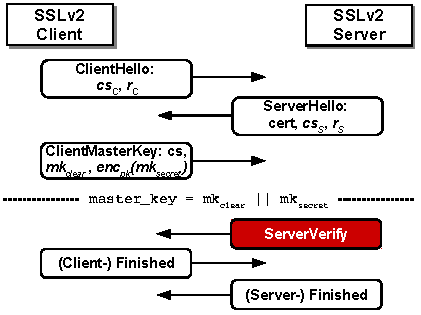
\includegraphics[width=\linewidth]{\DrownFigures/ssl-handshake} 
	\caption{\textbf{\ssltwo handshake.} The server responds with a \texttt{ServerVerify} message directly after receiving an RSA-\PKCS ciphertext contained in \texttt{ClientMasterKey}. This protocol feature enables our attack.\looseness=-1}
	\label{fig:ssl-handshake}
\end{figure}
%\fi
%
A client initiates an \ssltwo handshake by sending a
\texttt{ClientHello} message, which includes a list of cipher
suites $cs_c$ supported by the client and a client nonce $r_c$,
termed \texttt{challenge}.
The server responds with a \texttt{ServerHello} message, which
contains a list of cipher suites $cs_s$ supported by the server,
the server certificate, and a server nonce $r_s$, termed
$\texttt{connection\_ID}$.

The client responds with a \texttt{ClientMasterKey} message, which
specifies a cipher suite supported by both peers and key data
used for constructing a \texttt{master\_key}. In order to support
\textit{export} cipher suites with 40-bit security (e.g.,
\texttt{SSL\_RC2\_128\_CBC\_EXPORT40\_WITH\_MD5}), the key data is
divided into two parts:
\begin{itemize}
	\item $mk_{clear}$: A portion of the \texttt{master\_key} sent in the \texttt{ClientMasterKey} message as plaintext (termed \texttt{clear\_key\_data} in the \ssltwo standard).
	\item $mk_{secret}$: A secret portion of the
          \texttt{master\_key}, encrypted with RSA \PKCS (termed \texttt{secret\_key\_data}). 
\end{itemize}
The resulting \texttt{master\_key} $mk$ is constructed by
concatenating these two keys: $mk = mk_{clear} || mk_{secret}$. For
40-bit export cipher suites, $mk_{secret}$ is five bytes in length.
For non-export cipher suites, the whole \texttt{master\_key} is
encrypted, and the length of $mk_{clear}$ is zero.

The client and server can then compute session keys from the reconstructed \texttt{master\_key} $mk$:

\vspace{-6pt}
\begin{center}
\begin{math}
	\texttt{server\_write\_key} = MD5(mk || ``0" || r_c || r_s) \linebreak	
	\texttt{client\_write\_key} = MD5(mk || ``1" || r_c || r_s)
\end{math}
\end{center}
\vspace{-6pt}

The server responds with a \texttt{ServerVerify} message
consisting of the \texttt{challenge} $r_c$ encrypted with the
\texttt{server\_write\_key}.  Both peers then exchange
\texttt{Finished} messages in order to authenticate to each other.

Our attack exploits the fact that the server always decrypts an RSA-\PKCS
ciphertext, computes the \texttt{server\_write\_key}, and \textit{immediately}
responds with a \texttt{ServerVerify} message.  The \ssltwo standard
implies this message ordering, but does not make it explicit.
However, we observed this behavior in every implementation we
examined.  Our attack also takes advantage of the fact that the
encrypted $mk_{secret}$ portion of the \texttt{master\_key} can vary
in length, and is only five bytes for export ciphers.

% I Merged SSLv2 description and key derivation, ther were some redundancies ...

%\subsubsection{The SSLv2 key derivation mechanism}
%
%Recall that the RSA decryption code on the server decrypts the received RSA ciphertext, and checks the validity of the resulting plaintext as per the PKCS \#1 format. If the plaintext is valid, the server extracts from it the unpadded data, and uses that data, along with other information exchanged thus far during the protocol run, as the key for the chosen symmetric cipher. More formally:
%
%\begin{itemize}
%	\item Let the data from the decrypted RSA plaintext, after padding is removed, be termed \texttt{secret\_key\_data}.
%	\item Recall that the client and server have already exchanged a client nonce, termed \texttt{challenge} in the protocol standard, and a server nonce, termed $\texttt{connection\_ID}$.
%	\item Assume, as is the case throughout this work, that the chosen symmetric cipher is either export RC4 with a 128-bit key, of which 40 bits are secret, or export RC2 with the same key sizes\footnote{details vary slightly, but are very similar for other ciphers}. Then the client should send, along with the RSA ciphertext, a portion of the symmetric key in cleartext, termed \texttt{clear\_key\_data}, where \texttt{clear\_key\_data} is 11 bytes long. The sent \texttt{secret\_key\_data} should be exactly 5 bytes long. Let $\texttt{master\_key} = \texttt{clear\_key\_data} | \texttt{secret\_key\_data}$, where in this context $|$ refers to the concatenation operator.
%	\item Now let
%
%$\texttt{server\_write\_key} = MD5(\texttt{master\_key} | "0" | \texttt{challenge} | \texttt{connection\_ID})$
%
%$\texttt{client\_write\_key} = MD5(\texttt{master\_key} | "1" | \texttt{challenge} | \texttt{connection\_ID})$
%
%where the $|$ operator again means concatenation, and "0" and "1" refer to the corresponding ascii characters.
%
%	\item The respective keys are then used by each party both as keys for the chosen symmetric cipher, and as MAC keys.
%\end{itemize}

%As was hinted in the previous subsection, once an RSA key exchange with PKCS \#1 is implemented, the question immediately arises of how to act given an invalid RSA plaintext - recall that any observable difference in the treatment of invalid messages exposes a Bleichenbacher oracle to the attacker.
%Most implementations, including openssl, employ a counter-mechanism that has become somewhat standard: If the RSA plaintext is invalid or is of a wrong length, generate a random sequence of bytes of the expected length, and treat that sequence of bytes as if that was the plaintext after padding removal.
%
%As an aside, we note this counter-mechanism entails the risk of a timing attack: If the random byte sequence generation takes a measurable amount of time, an attacker may be able to observe the difference in processing times, and deduce the validity of the plaintext. Therefore, this counter-mechanism should be carefully implemented so as to require constant processing time. This is usually done by generating the random byte sequence before the RSA decryption, and choosing between the random sequence and the RSA plaintext according to the validity of the PKCS \#1 formatting. In fact, openssl's implementation of this mechanism was originally not constant-time for SSLv2, but the implementation was appropriately changed after we drew the maintainers' attention to this problem.



\ifsubmit\relax\else
\begin{figure}
	%\centering 
	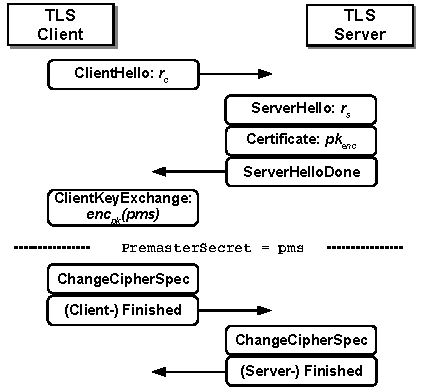
\includegraphics[width=\linewidth]{\DrownFigures/tls-handshake} 
	\caption{\textbf{TLS-RSA handshake.} After receiving an encrypted \pms, the server waits for an authenticated \texttt{ClientFinished} message.}
	\label{fig:tls-handshake}
\end{figure}
\fi

\paragraph{The TLS handshake protocol.}
In TLS~\cite{rfc5246} or \sslthree, the client initiates the handshake with a \texttt{ClientHello}, which contains a client random $r_c$ and a list of supported cipher suites. The server chooses one of the cipher suites and responds with three messages, \texttt{ServerHello}, \texttt{Certificate}, and \texttt{ServerHelloDone}. These messages include the server's choice of cipher suite, server nonce $r_s$, and a server certificate with an RSA public key. The client then uses the public key to encrypt a newly generated 48-byte \pms $pms$ and sends it to the server in a \texttt{ClientKeyExchange} message. The client and server then derive encryption and MAC keys from the \pms and the client and server random nonces. The details of this derivation are not important to our attack.  The client then sends \texttt{ChangeCipherSpec} and \texttt{Finished} messages. The \texttt{Finished} message authenticates all previous handshake messages using the derived keys. The server responds with its own \texttt{ChangeCipherSpec} and \texttt{Finished} messages.

The two main details relevant to our attacks are:
\begin{itemize}
	\item The \pms is always 48 bytes long, independent of the chosen cipher suite.  This is also true for export cipher suites.
	\item After receiving the \texttt{ClientKeyExchange} message, the server waits for the \texttt{ClientFinished} message, in order to authenticate the client.
\end{itemize}


\ifsubmit\relax\else
\subsubsection{Real-world protocol support}
TLSv1.0 is the most commonly supported protocol version, according to several surveys.  The SSL Labs SSL Pulse survey~\cite{ssllabs} reports that 98.6\% of about 140,000 popular TLS/SSL-enabled web sites supported TLSv1.0 in January 2016.  72.0\% supported TLSv1.2.  Support for \ssltwo was at 9.3\%, and \sslthree was at 29\%. Mayer et al.~\cite{DBLP:journals/corr/MayerZSH15} performed Internet-wide surveys of SMTP, IMAP, and POP3 between April and August 2015, and found that support for \ssltwo support was as high as 41.7\% of servers for SMTP on port 25 and as low as 3.7\% of IMAP servers on port 143.  Support for TLSv1.0 was nearly universal on these ports, varying from 91.6\% on port 25 to 98.9\% on port 143.

Bowen~\cite{bowencab} collected 213 million SSL/TLS client hellos and user agent strings from connections to popular sites, of which 183,000 (0.09\%) client hellos supported \ssltwo.  All of these client hellos also supported at least TLSv1.0.

Holz et al.~\cite{2016holz_analysis_tls-based_protocols_electronic_communication} performed passive monitoring to collect information about 16 million SSL/TLS connections during one week in July-August 2015.  They did not report any numbers for \ssltwo, and stated in personal communication that they did not observe any \ssltwo connections in their dataset.
\fi

%In response to our disclosure, OpenSSL has disabled \ssltwo by default in the 1.0.1r and 1.0.2f releases~\cite{opensslchangelog}.  

%This bug was also fixed in the aforementioned openssl releases.

\subsection{Bleichenbacher's attack}
\label{sec:bleichenbacher}
Bleichenbacher's attack is a padding oracle attack---it exploits the
fact that RSA ciphertexts should decrypt to \PKCS-compliant plaintexts.
If an implementation receives an RSA
ciphertext that decrypts to an invalid \PKCS plaintext, it might
naturally leak this information via an error message, by closing the
connection, or by taking longer to process the error condition.  This
behavior can leak information about the plaintext that can be modeled
as a cryptographic \textit{oracle} for the decryption
process. Bleichenbacher~\cite{Bleichenbacher} demonstrated how such an
oracle could be exploited to decrypt RSA ciphertexts.

%For example, the decrypting code may require different processing times for valid vs.\ invalid plaintexts - this is termed a "timing side-channel vulnerability". As another example, the decrypting code may send messages derived in some way from the plaintexts - this is termed a "direct message side channel vulnerability".
%The seminal work in this area \cite{Bleichenbacher} identified the general potential for such vulnerabilities, specifically using a direct message side channel vulnerability present in TLS implementations at the time, and demonstrated how such information could be gradually combined to eventually decrypt the RSA ciphertext in full.

\paragraph{Algorithm.}
In the simplest attack scenario, the attacker has a valid \PKCS
ciphertext $c_{0}$ that they wish to decrypt to discover the message
$m_{0}$.  They have no access to the private RSA key, but instead have
access to an oracle $\Oracle$ that will decrypt a ciphertext $c$ and
inform the attacker whether the most significant two bytes match
the required value for a correct \PKCS padding:
\begin{equation*} 
\Oracle(c) =  
\begin{cases} 
1 & \text{ if } m=c^d \bmod N \text{ starts with \hexb{00}{02}} \\ 
0 & \text{ otherwise.} 
\end{cases} 
\end{equation*} 

If the oracle answers with \texttt{1}, the attacker knows that $2B
\leq m \leq 3B-1$, where $B = 2^{8(\ell_m-2)}$.  The attacker can
take advantage of RSA malleability to generate new candidate ciphertexts
for any $s$:
\[
c = (c_{0} \cdot s^e) \bmod N = (m_{0} \cdot s)^e \bmod N 
\]
The attacker queries the oracle with $c$. If the oracle responds with
$0$, the attacker increments $s$ and repeats the previous
step. Otherwise, the attacker learns that for some~$r$, $2B \leq m_{0}s - rN  < 3B$. This allows the attacker to reduce the range of possible solutions to:  
\[ 
\frac{2B+rN}{s} \leq m_{0} < \frac{3B+rN}{s}  
\] 
The attacker proceeds by refining guesses for $s$ and $r$ values and
successively decreasing the size of the interval containing $m_{0}$.  At
some point the interval will contain a single valid value, $m_{0}$.
Bleichenbacher's original paper describes this process in further
detail~\cite{Bleichenbacher}.

\paragraph{Countermeasures.}
In order to protect against this attack, the decrypter must not leak
information about the \PKCS validity of the ciphertext.  The
ciphertext does not decrypt to a valid message, so the
decrypter generates a fake plaintext and continues the
protocol with this decoy.  The attacker should not be able to
distinguish the resulting computation from a correctly decrypted
ciphertext.

In the case of SSL/TLS, the server generates a random \pms to continue
the handshake if the decrypted ciphertext is
invalid.  The client will not possess the session key to send a valid
\texttt{ClientFinished} message and the connection will terminate.



\section{Breaking TLS with SSLv2}
In this section, we describe our cross-protocol DROWN attack that uses an
\ssltwo server as an oracle to efficiently decrypt TLS connections. The
attacker learns the session key for targeted TLS connections but does not
learn the server's private RSA key. We first describe our techniques using a
generic \ssltwo oracle. In Section~\ref{vulnerability}, we show how a
protocol flaw in \ssltwo can be used to construct such an oracle, and
describe our general DROWN attack. In Section~\ref{sec:special}, we show how
an implementation flaw in common versions of OpenSSL leads to a more powerful
oracle and describe our efficient special DROWN attack.

%\subsection{An efficient Bleichenbacher attack}

%\subsection{Attack scenario}
\label{sec:attack-scenario}

We consider a server accepting TLS connections from clients. The connections are established using a secure, state-of-the-art TLS version (1.0--1.2) and a \texttt{TLS\_RSA} cipher suite with a private key unknown to the attacker.

%\paragraph{Server RSA key exposed via \ssltwo.}
The same RSA public key as the TLS connections is also used for \ssltwo. For
simplicity, we will refer to the servers accepting TLS and \ssltwo
connections as the same entity.

%\paragraph{The attacker's position in the network.}
Our attacker is able to passively eavesdrop on traffic between the client and
server and record RSA-based TLS traffic.
The attacker may or may not be also required to perform active man-in-the-middle
interference, as explained below.

The attacker can expect to decrypt one out of 1,000 intercepted TLS
connections in our attack for typical parameters. This is a devastating
threat in many scenarios. For example, a decrypted TLS connection might
reveal a client's HTTP cookie or plaintext password, and an attacker would
only need to successfully decrypt a single ciphertext to compromise the
client's account. In order to collect 1,000 TLS connections, the attacker
might simply wait patiently until sufficiently many connections are recorded.
A less patient attacker might use man-in-the-middle interference, as in the
BEAST attack~\cite{beast-2011}.

\ifext
In order to collect 1,000 TLS connections, the attacker might simply wait patiently until sufficiently many connections are recorded.  If the attacker's intended victim is the \emph{server}, rather than a specific client, observing this many connections from many clients might take only a short time for an attacker who is located at a company firewall or who could perform a DNS spoofing or BGP hijacking attack to redirect traffic transparently through themselves.  If the attacker's intended victim is a \emph{particular client}, this is still feasible in many cases.  As an example, the Mozilla Thunderbird email client will check for new email messages every ten minutes by default.  A targeted user will make 1,000 connections after leaving the application running for a week.

A less patient attacker might have to resort to active man-in-the-middle techniques
in order to collect the required 1,000 TLS connections.
The attacker could embed or inject malicious JavaScript on an otherwise innocuous web site to cause the client to connect repeatedly to the victim server in a short time frame, as in the BEAST attack~\cite{beast-2011}.
The attacker may also need to trigger an error in each of the connections, in order
to prevent the handshakes from using TLS session resumption.
\fi


\subsection{A generic \ssltwo oracle}

Our attacks make use of an oracle that can be queried on a ciphertext and leaks information about the decrypted plaintext; this abstractly models the information gained from an \ssltwo server's behavior.  Our \ssltwo oracles reveal many bytes of plaintext, enabling an efficient attack.

Our cryptographic oracle $\Oracle$ has the following functionality: 
$\Oracle$ decrypts an RSA ciphertext $c$ and responds with ciphertext validity based on the decrypted message $m$.  
The ciphertext is valid only if $m$ starts with \hexb{00}{02} followed by non-null padding bytes, a delimiter byte \hex{00}, and a \texttt{master\_key} $mk_{secret}$ of correct byte length $\ell_k$.
We call such a ciphertext \textit{\sslconform}.

All of the \ssltwo padding oracles we instantiate give the attacker similar information about a \PKCSconform \ssltwo ciphertext:
\begin{equation*} 
\Oracle(c) =  
\begin{cases} 
mk_{secret} & \text{ if } c^d \bmod N = 00 || 02 || PS || 00 || mk_{secret}  \\ 
0 & \text{ otherwise.} 
\end{cases} 
\end{equation*}
That is, the oracle $\Oracle(c)$ will return the decrypted message $mk_{secret}$ if it is queried on a \PKCSconform \ssltwo ciphertext $c$ corresponding to a correctly \PKCS padded encryption of $mk_{secret}$.  The attacker then learns $\ell_k + 3$ bytes of $m = c^d \bmod N$: the first two bytes are $00 || 02$, and the last $\ell_k+1$ bytes are $00 || mk_{secret}$.  The length $\ell_k$ of $mk_{secret}$ varies based on the cipher suite used to instantiate the oracle.  For export-grade cipher suites such as \texttt{SSL\_RSA\_EXPORT\_WITH\_RC2\_CBC\_40\_MD5},
%or \texttt{SSL\_RSA\_EXPORT\_WITH\_RC4\_40\_MD5}\@,
$k$ will be 5 bytes, so the attacker learns 8 bytes of $m$.

\subsection{DROWN attack template}
\label{sec:adapted-bb-compact}
Our attacker will use an \ssltwo oracle $\Oracle$ to decrypt a TLS \texttt{ClientKeyExchange}.  
The behavior of $\Oracle$ poses two problems for the attacker. First, a TLS key exchange ciphertext decrypts to a 48-byte \pms. But since no \ssltwo cipher suites have 48-byte key strengths, this means that a valid TLS ciphertext is invalid to our oracle $\Oracle$. 
In order to apply Bleichenbacher's attack, the attacker must transform the TLS ciphertext into a valid \ssltwo key exchange message. Second, $\Oracle$ is very restrictive, since it strictly checks the length of the unpadded message. 
According to Bardou et al.~\cite{efficient-padding-oracle-2012}, Bleichenbacher's attack would require 12 million queries to such an oracle.\footnote{See Table~1 in~\cite{efficient-padding-oracle-2012}. The oracle is denoted with the term \texttt{FFF}.} 
%As each query would require an exhaustive search over $2^{40}$ values, this would make the attack significantly more costly.

Our attacker overcomes these problems by following this generic attack flow:
\begin{enumerate}
 \setcounter{enumi}{-1}
	\item The attacker collects many encrypted TLS RSA key exchange messages.
	\item The attacker converts one of the intercepted TLS ciphertexts containing a 48-byte \pms to an RSA \PKCS encoded ciphertext valid to the \ssltwo oracle $\Oracle$. \ifext We accomplish this by taking advantage of RSA ciphertext malleability and a technique of Bardou et al.~\cite{efficient-padding-oracle-2012}. \fi
	\item Once the attacker has obtained a valid \ssltwo RSA ciphertext, they can continue with a modified version of Bleichenbacher's attack, and decrypt the message after many more oracle queries.
	\item The attacker then transforms the decrypted plaintext back into the original plaintext, which is one of the collected TLS handshakes.
\end{enumerate}

We describe the algorithmic improvements we use to make each of these steps efficient below.

\subsubsection{Finding an \sslconform ciphertext}
\label{sec:trimmers}
The first step for the attacker is to transform the original TLS \texttt{ClientKeyExchange} message $c_0$ from a \tlsconform ciphertext into an \sslconform ciphertext. 
\ifext
A trivial approach would be to generate multipliers $s_i \in \{s_1,s_2,\ldots\}$, and compute ciphertexts $c_i = (c_0 {s_i}^e) \bmod N$, until one gets accepted by $\Oracle$.
However, the number of generated ciphertexts would be high, because $\Oracle$ is very restrictive; for 2048-bit RSA keys and an oracle expecting a 5-byte $mk_{secret}$ the probability that a random ciphertext becomes \sslconform is $P_{rnd} \approx (1/256)^3 * (255/256)^{249} \approx 2^{-25}$.
\fi

For this task, we rely on the concept of \emph{trimmers}, which were introduced by Bardou et al.~\cite{efficient-padding-oracle-2012}. 
Assume that the message $m_{0} = {c_0}^d \bmod N$ is divisible by a small number~$t$. In that case,  $m_{0} \cdot t^{-1} \bmod{N}$ simply equals the natural number $m_{0} / t$. 
If we choose $u \approx t$, and multiply the original message by $u \cdot t^{-1}$, the resulting number will lie near the original message: $m_0 \approx m_0 / t \cdot u$.  \ifext We shall refer to such fractions as ``small'' fractions. \fi

This method gives a good chance of generating a new \sslconform message. 
Let $c_0$ be an intercepted \tlsconform RSA ciphertext, and let $m_0 = c_0^d \bmod N$ be the \ifext corresponding \fi plaintext.  We select a multiplier $s = u/t \bmod N = u t^{-1} \bmod N$ where $u$ and $t$ are coprime, compute the value $c_1 = c_0 s^e \bmod N$, and query $\Oracle(c_1)$.  We will receive a response if $m_1 = m_0 \cdot u/t$ is \sslconform.  

As an example, let us assume a 2048-bit RSA ciphertext with $\ell_k = 5$, and consider the fraction $u = 7, t = 8$.  The probability that $c_0 \cdot u/t$ will be \sslconform is 1/7,774, so we expect to make 7,774 oracle queries before obtaining a positive response from $\Oracle$. Appendix~\ref{sec:fraction-probability} gives more details on computing these probabilities.

\subsubsection{Shifting known plaintext bytes}
\label{sec:rotations}
Once we have obtained an \sslconform ciphertext $c_1$, the oracle has also revealed the $\ell_k+1$ least significant bytes ($mk_{secret}$ together with the delimiter byte \hex{00}) and two most significant \hexb{00}{02} bytes of the \sslconform message $m_1$.  We would like to \emph{rotate} these known bytes around to the right, so that we have a large block of contiguous known most significant bytes of plaintext.
In this section, we show that this can be accomplished by multiplying by some shift $2^{-r} \bmod N$.  In other words, given an \sslconform ciphertext $c_1 = m_1^e \bmod N$, we can efficiently generate an \sslconform ciphertext $c_2 = m_2^e \bmod N$ where $m_2 = s \cdot m_1 \cdot 2^{-r} \bmod N$ and we know several most significant bytes of $m_2$. 

Let $R = 2^{8(k+1)}$ and $B = 2^{8(\ell_m-2)}$. Abusing notation slightly, let the integer $m_1 = 2 \cdot B + PS \cdot R + mk_{secret}$ be the plaintext satisfying $m_1^e = c_1 \bmod N$.  At this stage, the $\ell_k$-byte integer $mk_{secret}$ is known and the $\ell_m-\ell_k-3$-byte integer $PS$ is not.

Let $\tilde{m_1} = 2 \cdot B + mk_{secret}$ be the known components of $m_1$, so $m_1 = \tilde{m_1} + PS \cdot R$. We can use this to compute a new plaintext for which we know many most significant bytes.  Consider the value:
\[
m_1 \cdot R^{-1} \bmod N = \tilde{m_1} \cdot R^{-1} + PS \bmod N.
\]
The value of $PS$ is unknown and consists of $\ell_m-\ell_k-3$ bytes.  This means that the known value $\tilde{m_1} \cdot R^{-1}$ shares most of its $\ell_k+3$ most significant bytes with $m_1 \cdot R^{-1}$.

Furthermore, we can iterate this process by finding a new multiplier $s$ such that $m_2 = s \cdot m_1 \cdot R^{-1} \bmod N$ is also \sslconform.  A randomly chosen $s < 2^{30}$ will work with probability $2^{-25.4}$.  We can take use the bytes we have already learned about $m_1$ to efficiently compute such an $s$ with only 678 oracle queries in expectation for a 2048-bit RSA modulus.   Appendix~\ref{sec:rotation-details} gives more details.

\subsubsection{Adapted Bleichenbacher iteration}
\label{sec:bb-iteration}
It is feasible for all of our oracles to use the previous technique to entirely recover a plaintext message.  However, for our \ssltwo protocol oracle it is cheaper after a few iterations to continue using Bleichenbacher's original attack.  We can apply the original algorithm proposed by Bleichenbacher as described in Section~\ref{sec:bleichenbacher}\ifext, with minimal modifications\fi.

Each step obtains a message that starts with the required \hexb{00}{02} bytes after two queries in expectation.
Since we know the value of the $\ell_k+1$ least significant bytes after multiplying by any integer, we can query the oracle only on multipliers that cause the $(\ell_k+1)$st least significant byte to be zero.  However, we cannot ensure that the padding string is entirely nonzero; for a 2048-bit modulus this will hold with probability 0.37.

For a 2048-bit modulus, the total expected number of queries when using this technique to fully decrypt the plaintext is $2048 * 2 / 0.37 \approx 11,000$.


%\ifext
\begin{figure}[t]
	%\centering 
	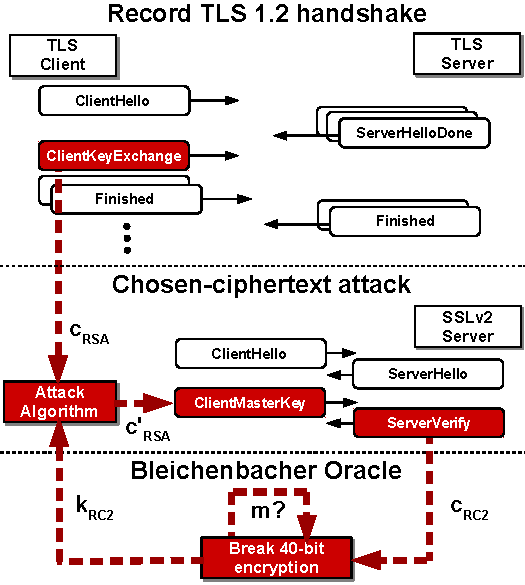
\includegraphics[width=\linewidth]{\DrownFigures/ssl-tls} 
	\caption{\textbf{\ssltwo-based Bleichenbacher attack on TLS}\,---\,%
	An attacker passively collects RSA ciphertexts from a TLS 1.2 handshake, and
    then performs oracle queries against a server that supports \ssltwo with the
	same public key to decrypt the TLS ciphertext.
	}
	\label{fig:ssl-tls}
\end{figure}
%\fi

\section{General DROWN} 
\label{vulnerability}

In this section, we describe how to use any correct \ssltwo implementation accepting export-grade cipher suites as a padding oracle.  We then show how to adapt the techniques described in Section~\ref{sec:adapted-bb-compact} to decrypt TLS RSA ciphertexts.

\subsection{The SSLv2 export padding oracle} 
\label{vulnerability}
\ssltwo is vulnerable to a direct message side channel vulnerability exposing a Bleichenbacher oracle to the attacker.
The vulnerability follows from three properties of \ssltwo.  First, the server immediately responds with a \texttt{ServerVerify} message after receiving the \texttt{ClientMasterKey} message, which includes the RSA ciphertext, without waiting for the \texttt{ClientFinished} message that proves the client knows the RSA plaintext.  Second, when choosing 40-bit export RC2 or RC4 as the symmetric cipher, only 5 bytes of the \texttt{master\_key} ($mk_{secret}$) are sent encrypted using RSA, and the remaining 11 bytes are sent in cleartext.  Third, a server
implementation that correctly implements the anti-Bleichenbacher countermeasure 
and receives an RSA key exchange message with invalid
padding will generate a random premaster secret and carry out the
rest of the TLS handshake using this randomly generated key material.

This allows an attacker to deduce the validity of RSA ciphertexts in the following manner:

\begin{enumerate}
	\item The attacker sends a \texttt{ClientMasterKey} message, which contains an RSA ciphertext $c_0$ and any choice of 11 clear key bytes for $mk_{clear}$. The server responds with a \texttt{ServerVerify} message, which contains the \texttt{challenge} encrypted using the \texttt{server\_write\_key}.
	\item The attacker performs an \textit{exhaustive search} over the possible values of the 5 bytes of the \texttt{master\_key} $mk_{secret}$, computes the corresponding \texttt{server\_write\_key}, and checks whether the \texttt{ServerVerify} message decrypts to \texttt{challenge}. One value should pass this check; call it $mk_0$. Recall that if the RSA plaintext was valid, $mk_0$ is the unpadded data in the RSA plaintext $c_0 ^d$. Otherwise, $mk_0$ is a randomly generated sequence of 5 bytes.
	\item The attacker re-connects to the server with the same RSA ciphertext $c_0$. The server responds with another \texttt{ServerVerify} message that contains the current \texttt{challenge} encrypted using the current \texttt{server\_write\_key}. If the decrypted RSA ciphertext was valid, the attacker can use $mk_0$ to decrypt a correct \texttt{challenge} value from the \texttt{ServerVerify} message. Otherwise, if the \texttt{ServerVerify} message does not decrypt to \texttt{challenge}, the RSA ciphertext was invalid, and $mk_0$ must have been random.
\end{enumerate}

Thus we can instantiate an oracle $\OracleSSLexp$ using the procedure above; each oracle query requires two server connections and $2^{40}$ decryption attempts in the simplest case.  For each oracle call $\OracleSSLexp(c)$, the attacker learns whether $c$ is valid, and if so, learns the two most significant bytes \hexb{00}{02}, the sixth least significant \hex{00} delimiter byte, and the value of the 5 least significant bytes of the plaintext $m$.

\ifext
If the server does not support 40-bit export ciphers, the attack can also be mounted in feasible computation time by choosing DES as the symmetric cipher.  Choosing DES means the exhaustive search is now done over a key space of 56 bits, thus increasing the cost of the attack by a factor of \begin{math} 2^{16} \end{math}, but does not fundamentally change anything except the increased cost.
\fi

\ifsubmit\relax\else
\subsection{OpenSSL special DROWN oracle}

We discovered a vulnerability present in OpenSSL versions prior to March 4, 2015 that allows a client to improperly provide cleartext key bytes for non-export ciphers.  Affected servers will substitute these bytes for bytes from the encrypted key.  This allows a client to successively learn a byte at a time of an encrypted key by brute forcing only 256 possibilities for each query. For a non-export 128-bit cipher suite such as \texttt{SSL\_RC4\_WITH\_MD5}, the attacker learns 19 bytes of the decrypted message.  We describe this vulnerability in more detail in Appendix~\ref{sec:clear-key-vuln}.  A client can then construct a Bleichenbacher oracle from this behavior by validating the \texttt{ServerVerify} message against the candidate key provided in the \texttt{clear\_key\_data}, resulting in no brute-force computation.
\fi

\subsection{TLS decryption attack}
\label{sec:bb-performance}

In this section, we describe how the oracle described in Section~\ref{vulnerability} can be used to carry out a feasible attack to decrypt passively collected TLS ciphertexts.

%\subsubsection{Attack scenario}
As described in Section~\ref{sec:attack-scenario}, we consider a server that accepts TLS connections from clients using an RSA public key that is exposed via \ssltwo, and an attacker who is able to passively observe these connections.

%\paragraph{Server supports export cipher suites for \ssltwo.}
We also assume the server supports export cipher suites for \ssltwo.
This can happen for two reasons.
First, the same server operators that fail to follow best practices in disabling \ssltwo~\cite{rfc6176} may also fail to follow best practices by supporting export cipher suites.
Alternatively, the server might be running a version of OpenSSL prior to January 2016, in which case it is vulnerable to the OpenSSL cipher suite selection bug described in Section~\ref{sec:openssl-selection}, and an attacker may negotiate a cipher suite of his choice independent of the server configuration.

% Nimrod: The previous subsection, introducing the generic SSLv2 oracle,
% already (implicitly) assumes this. Since we're short on space, I vote
% to remove this, at least for now.
\ifext
\paragraph{Correct Bleichenbacher countermeasure.}
We assume the server implements the recommended countermeasure against Bleichenbacher's attack in all protocol versions, including \ssltwo. If the decrypted RSA ciphertext has invalid padding, the server generates a random \pms or \texttt{master\_key} and continues the handshake with this random string. We assume this countermeasure is implemented correctly and the server is neither vulnerable to timing nor flush-and-reload side-channel attacks~\cite{Meyer14,Zhang:2014:CSA:2660267.2660356}.
\fi

%\paragraph{Computing power.}
The attacker needs access to computing power sufficient to perform a $2^{50}$ time attack, mostly brute forcing symmetric key encryption.  After our optimizations, this can be done with a one-time investment of a few thousand dollars of GPUs, or in a few hours for a few hundred dollars in the cloud.  Our cost estimates are described in~Section~\ref{sec:ec2_results}.

\if0
In our simplest attack scenario, an attacker is passively observing many connections between modern clients and server who negotiate a secure TLS version (1.0--1.2) with an RSA cipher suite and a well-generated, secure RSA public key.   The server is also configured to support \ssltwo with the same certificate as in TLS if a client requests it, although the modern victim clients will never negotiate \ssltwo.  The server implements the recommended countermeasures against Bleichenbacher attacks described in Section~\ref{sec:bleichenbacher}.



Our attacker will use our SSLv2 oracle $\OracleSSL$ to decrypt a TLS \texttt{ClientKeyExchange}.  We specialize the discussion below to our protocol-level oracle described in Section~\ref{vulnerability} and refer to this attack as the \emph{general} DROWN attack.  The adaptations to the OpenSSL clear-key oracle, which produces our faster \emph{special} DROWN attack are similar and are described in Section~\ref{sec:special}.
\fi

\subsubsection{Constructing the attack}

The attacker can exploit the \ssltwo vulnerability
\ifext as illustrated in Figure~\ref{fig:ssl-tls}, \fi
following the generic attack outline described in Section~\ref{sec:adapted-bb-compact},
consisting of several distinct phases:

\begin{enumerate}
 \setcounter{enumi}{-1}
	\item The attacker passively collects 1,000 TLS handshakes from
	connections using RSA key exchange.

	\item They then attempt to convert the intercepted TLS ciphertexts containing a 48-byte \pms to valid RSA \PKCS encoded ciphertexts containing five-byte messages using the fractional trimmers described in Section~\ref{sec:trimmers}, and querying $\OracleSSLexp$. The attacker sends the modified ciphertexts to the server using fresh \ssltwo connections with weak symmetric ciphers and uses the \texttt{ServerVerify} messages to deduce ciphertext validity as described in the previous section. For each queried RSA ciphertext, the attacker must perform a brute force attack on the weak symmetric cipher. The attacker expects to obtain a valid \ssltwo ciphertext after roughly 10,000 oracle queries, or 20,000 connections to the server.

	\item Once the attacker has obtained a valid \ssltwo RSA ciphertext
	$c_1 = m_1^e$, they use the shifting technique explained in
	Section~\ref{sec:rotations} to find an integer $s_1$ such that
	$m_2 = m_1 \cdot 2^{-40} \cdot s_1$ is also \sslconform.
	Appendix~\ref{sec:general-rotations} contains more details on this step.

	\item The attacker then applies the shifting technique again to find
	another integer $s_2$ such that $m_3 = m_2 \cdot 2^{-40} \cdot s_2$
	is also \sslconform.

	\item They then search for yet another integer $s_3$ such that
	$m_3 \cdot s_3$ is also \sslconform.

	\item Finally, the attacker can continue with our adapted Bleichenbacher
	iteration technique described in Section~\ref{sec:bb-iteration}, and
	decrypts the message after an expected 10,000 additional oracle queries,
	or 20,000 connections to the server.

	\item The attacker can then transform the decrypted plaintext back into
	the original plaintext, which is one of the 1,000 intercepted TLS 		handshakes.

\end{enumerate}

\paragraph{The rationale behind the different phases.}
Bleichenbacher's original algorithm requires a conformant message $m_0$, and a multiplier $s_1$ such that $m_1 = m_0 \cdot s_1$ is also conformant.
Na\"{\i}vely, it would appear we can apply the same algorithm here, after completing Phase 1.
However, the original algorithm expects $s_1$ to be of size about $2^{24}$. This is not the case when we use fractions for $s_1$, as the integer $s_1 = u t^{-1} \bmod N$ will be the same size as $N$.

Therefore, our approach is to find a conformant message for which we know the 5 most significant bytes; this will happen after multiple rotations and
this message will be $m_3$.
After finding such a message, finding $s_3$ such that $m_4 = m_3 \cdot s_3$ is also conformant becomes trivial.
From there, we can finally apply the adapted Bleichenbacher iteration technique as described in Appendix~\ref{sec:general-bleichenbacher}.

\begin{table}[t]
  \centering
	\begin{tabular}{rrrrrr}
	\toprule
	\textbf{Optimizing} & \textbf{Cipher-} & \textbf{$|F|$}     & \textbf{\ssltwo}  & \textbf{Offline} \\
        \textbf{for}        & \textbf{texts}   &           & \textbf{connections} & \textbf{work} \\
	\midrule
	offline work        &           12,743 &          1 &            50,421  & $2^{49.64}$ \\
        offline work        &            1,055 &         10 &              46,042  & $2^{50.63}$ \\
	% compromise is achieved by using fractions {8/7, 8/9}; numbers are now final
       	compromise          &            4,036 &          2 &              41,081  & $2^{49.98}$ \\
	online work         &            2,321 &          3 &              38,866  & $2^{51.99}$ \\
	online work         &              906 &          8 &              39,437  & $2^{52.25}$ \\
	\bottomrule
	\end{tabular}
		\caption{\textbf{2048-bit Bleichenbacher attack complexity}\,---\,%
		The cost to decrypt one ciphertext can be adjusted by choosing the set of
        fractions $F$ the attacker applies to each of the passively collected
		ciphertexts in the first step of the attack. This choice affects several
		parameters: the number of these collected ciphertexts, the number of
 		connections the attacker makes to the \ssltwo server, and the number of
		offline decryption operations.
		}
        \label{tab:reasonable_parameters}
\end{table}

\begin{table}[t]
\begin{tabular*}{\linewidth}{@{\extracolsep{\fill}\hskip\tabcolsep}rrrrr}
\toprule
\textbf{Key size}    & \textbf{Phase 1} & \textbf{Phases 2--5} & \textbf{Total}   & \textbf{Offline} \\
                     &                 &                 & \textbf{queries} & \textbf{work}    \\
\midrule
% This is all when using 4/5, which has a maximal "native probability" of 0.1.
% Offline work is always step1 * 2**38
%              1024 &  (0.1 * 0.62 * 1/256)**(-1)  & + 256 / 0.62 * 2 + 2/0.62 + 1024 * 2 / 0.62
               1024 &  4,129   &  4,132  &  8,261 & $2^{50.01}$ \\

%              2048 & (0.1 * 0.37 * 1/256)**(-1)   & + (2.72 * 2**8) * 2 + 2.72*2 + 2048 * 2 / 0.37 (number for phase 5 also matches runs)
               2048 &  6,919   &  12,468 & 19,387 & $2^{50.76}$ \\

%              4096 & (0.1 * 0.14 * 1/256)**(-1)   & + 2**8 / 0.14 * 2 + 2/0.14 + 4096 * 2 / 0.14
               4096 &  18,286  &  62,185 & 80,471 & $2^{52.16}$ \\
\bottomrule
\end{tabular*}
	\caption{\textbf{Oracle queries required by our attack}\,---\,%
	In Phase 1, the attacker queries the oracle until an \ssltwo conformant
	ciphertext is found. In Phases 2--5, the attacker decrypts this ciphertext
	using leaked plaintext. These numbers minimize total queries. In our attack,
	an oracle query represents two server connections.
	}
	\label{tab:optimal_queries}
\end{table}

\newcommand{\GPUTable}{
\begin{table*}[t]
 \centering
 \begin{tabular}{llrrrr}
        \toprule
        \textbf{Platform} & \textbf{Hardware} & \textbf{Cost} & \textbf{Full attack}  & \textbf{Cost to perform attack in 1 day} \\
        \midrule
        Na\"{\i}ve CPU & 4 Intel Xeon E7-4820 & $\$21,400$ & $114$ days  & \$$2,440,000$\\
        Na\"{\i}ve GPU & ZOTAC GeForce GTX TITAN & $\$2,400$  & $189$ days & \$$450,000$ \\
        Na\"{\i}ve FPGA & 64 Spartan-6 LX150 & $\$60,000$ & $51.5$ days  & \$$3,090,000$  \\
        \cmidrule{1-5}
        Optimized Hashcat & NVIDIA GTX / AMD R9 & \$18,040 & $0.75$ days & \$13,500 \\
        Optimized EC2 & NVIDIA & \$440 & $0.33$ days & \$147 \\
        \bottomrule
    \end{tabular}	
	\caption{\textbf{Time and cost efficiency of our attack on different hardware platforms.}\,---\,%
	The brute force attacks against symmetric export keys are the most expensive
	part of our attack. We compared the performance of a na\"{\i}ve
	implementation of our attack on different platforms, and decided that a GPU
	implementation held the most promise. We then heavily optimized our GPU
	implementation, obtaining several orders of magnitude in speedup.
	}
\label{perf_comparison}
\end{table*}
}

\subsubsection{Attack performance}
The attacker wishes to minimize three major costs in the attack: the number of recorded ciphertexts from the victim client, the number of connections to the victim server, and the number of symmetric keys to be brute forced.
The requirements for each of these elements are governed by the set of fractions to be multiplied with each RSA ciphertext in the first phase, as described in Section~\ref{sec:trimmers}.

Table~\ref{tab:reasonable_parameters} highlights a few choices for $F$ and the resulting performance metrics for 2048-bit RSA keys.
Appendix \ref{sec:adapted-bb} provides more details on the derivation of these numbers and other optimization choices.
Table \ref{tab:optimal_queries} gives the expected number of Bleichenbacher queries for different RSA key sizes, when minimizing total oracle queries.

%These are fractions of small coprime numbers, similar to the example $u/t = 8/7$, and ideally amenable to the additional optimization described above.





%The special DROWN attack requires similar numbers of ciphertexts and oracle queries, but the amount of computation is negligible.




\subsection{Implementing general DROWN with GPUs} 
%% In the following section, we experimentally evaluate the cost of brute forcing export \texttt{master\_key} values on CPU, GPU, FPGA, and cloud computing platforms. 
%% We then experimentally evaluate our general DROWN attack using the 
%% \texttt{SSL\_RC2\_128\_CBC\_EXPORT40\_WITH\_MD5}
%% cipher suite, which is the most suitable for this attack.

%% \subsubsection{Comparing hardware platforms}
\if0
The most computationally expensive part of our general DROWN attack is breaking the 40-bit symmetric key.  We wanted to find the platform that would have the best tradeoff of cost and speed for the attack, so we performed some preliminary experiments comparing performance of symmetric key breaking on CPUs, GPUs, and FPGAs.  These experiments used a na\"{\i}ve version of the attack using the OpenSSL implementation of MD5 and RC2.

The CPU machine contained four Intel Xeon E7-4820 CPUs with a total of 32 cores (64 concurrent threads). The GPU system was equipped with a ZOTAC GeForce GTX TITAN and an Intel Xeon E5-1620 host CPU\@. The FPGA setup consisted of 64 Spartan-6 LX150 FPGAs.

We benchmarked the performance of the CPU and GPU implementations over a large corpus of randomly generated keys, and then extrapolated to the full attack.
For the FPGAs, we tested the functionality in simulation and estimated the actual runtime by theoretically filling the FPGA up to 90\% with the design, including communication.
Table~\ref{perf_comparison} compares the three platforms.

While the FPGA implementation was the fastest in our test setup, the speed-to-cost ratio of GPUs was the most promising. Therefore, we decided to focus on optimizing the attack on the GPU platform.
\fi

\ifext
\subsubsection{Optimized GPU implementation}
\label{sec:gpu_brief}
We developed a highly optimized GPU implementation of our general DROWN brute force attack.  Our first na\"{\i}ve GPU implementation performed around 26MH/s, where MH measures the calculation of an MD5 hash and the RC2 decryption. The optimizations described below gave a final speed of 515MH/s, a speedup factor of 19.8.
\fi

\ifext
We obtained our improvements through a number of optimizations.  Our original implementation ran into a communication bottleneck in the PCI-E bus in transmitting candidate keys from CPU to GPU, so we removed this bottleneck by generating key candidates on the GPU itself.  We optimized memory management, including storing candidate keys and the RC2 permutation table in constant memory, which is almost as fast as a register, instead of slow global memory.  We optimized the cryptographic checks themselves by rewriting the RC2 implementation to use 32-bit instructions, removing unnecessary RC2 keysize checks, dropping unused ADD instructions during MD5, and manually shifting input bytes into the MD5 input registers to avoid loop branches.
\looseness=1
\fi

\ifext

\label{sec:ec2_results}
%In this section, we discuss attack performance and cost when a rented cloud compute cluster is used for the GPU breaking.
\fi

The most computationally expensive part of our general DROWN attack is breaking the 40-bit symmetric key, so we developed a highly optimized GPU implementation of this brute force attack.  Our first na\"{\i}ve GPU implementation performed around 26MH/s, where MH denotes the time required for testing one million possible values of $mk_{secret}$. Our optimized implementation runs at a final speed of 515MH/s, a speedup factor of 19.8.  
\label{sec:gpu_brief}

We obtained our improvements through a number of optimizations.  For example, our original implementation ran into a communication bottleneck in the PCI-E bus in transmitting candidate keys from CPU to GPU, so we removed this bottleneck by generating key candidates on the GPU itself.  We optimized memory management, including storing candidate keys and the RC2 permutation table in constant memory, which is almost as fast as a register, instead of slow global memory. 
\ifext  We optimized the cryptographic checks themselves by rewriting the RC2 implementation to use 32-bit instructions, removing unnecessary RC2 keysize checks, dropping unused ADD instructions during MD5, and manually shifting input bytes into the MD5 input registers to avoid loop branches.  We describe these optimizations in further detail in Appendix~\ref{sec:gpu}. \fi

We experimentally evaluated our optimized implementation on a local cluster and in the cloud.
We used it to execute a full attack of $2^{49.6}$ tested keys on each platform.
The required number of keys to test during the attack is a random variable, distributed geometrically, with an expectation that ranges between $2^{49.6}$ and $2^{52.5}$ depending on the choice of optimization parameters.
We treat a full attack as requiring $2^{49.6}$ tested keys overall.

\paragraph{Hashcat.}
Hashcat~\cite{hashcat} is an open source optimized password-recovery tool.
The Hashcat developers allowed us to use their GPU servers for our attack evaluation. 
The servers contain a total of 40 GPUs: 32 Nvidia GTX 980 cards, and 8 AMD R9 290X cards.
The value of this equipment is roughly \$18,040.
Our full attack took less than 18 hours to complete on the Hashcat servers, with the longest single instance taking 17h9m.

% Nimrod: Generally, we can't report times which are different from wallclock times without further explanation,
% like "retroactively assuming a perfecly balanced distribution..."
% The instance that took longest took 1029m41.176, which is 17.16 hours,
% so I think any number smaller than 18 hours would need to be discussed.

\paragraph{Amazon EC2.}
\label{sec:ec2_results}
% AH: Suggest trimming this as in the submitted version
\ifext
% !TEX root = ../../../proposal.tex
%\section{Brute Forcing Keys with Amazon EC2} 
\label{sec:ec2-details}

%Amazon Elastic Cloud Compute (EC2)~\cite{ec2} is a service that provides on-demand virtualized compute resources to customers. 
%This is an affordable alternative to provisioning one's own local cluster.

Amazon EC2 billing is based on the \textit{instance-hour}. An \textit{instance} represents a single virtualized machine and its associated cores, memory, and storage. For our experiments we used \texttt{g2} instances, which are equipped with high-performance NVIDIA GPUs, each with 1,536 CUDA cores. The two available models for this instance type are the \texttt{g2.2xlarge} and the \texttt{g2.8xlarge}, containing one and four GPUs, respectively.

It is possible to request instances at a fixed on-demand rate, or bid on instances at the discounted spot instance rate. Spot instances may be terminated depending on demand, but the savings in cost are significant compared to the on-demand rate. 
When we ran our experiments in January 2016, the on-demand rate for the \texttt{g2.2xlarge} model was \$0.65/hr and the rate for the \texttt{g2.8xlarge} model was \$2.65/hr, while the average spot rates we paid were \$0.09/hr and \$0.83/hr respectively.

We used a cluster composed of 200 spot instances: 150 \texttt{g2.2xlarge} which contain one GPU and 50 \texttt{g2.8xlarge}, each containing four GPUs, spread across multiple availability zones within the US-East region.
This distribution was determined by price: we were not able to launch more than 50 \texttt{g2.8xlarge} instances without a sharp spike in spot prices. We used the optimized Hashcat implementation on the same workload of key requests as the experiments run on the Hashcat servers.  We used Slurm~\cite{yoo2003slurm} to distribute jobs across compute nodes.

The GPU breaking experiment completed successfully, with two minor caveats. First, the 150 \texttt{g2.2xlarge} nodes completed their workloads at the 6h26m mark, while the other 50 \texttt{g2.8xlarge} nodes did not finish until the 7h41m mark. More careful job distribution would ensure that all nodes completed at approximately the same time, reducing the overall runtime. Second, in this particular run, $7.2\%$ of the jobs that we expected to complete were terminated early due to overheating GPUs.  The attack was successful despite the failed jobs, so we did not rerun them. In a more carefully engineered implementation, the unfinished jobs could have been reallocated to the unused GPU capacity without increasing the overall runtime.

The total cost of the experiment was \$440, and terminated in under 8 hours including startup and shutdown.


\else
We also ran our optimized GPU code on the Amazon Elastic Compute Cloud (EC2) service.  We used a cluster composed of 200 variable-price ``spot'' instances: 150 \texttt{g2.2xlarge} instances, each containing one high-performance NVIDIA GPU with 1,536 CUDA cores and 50 \texttt{g2.8xlarge} instances, each containing four of these GPUs.  
When we ran our experiments in January 2016, the average spot rates we paid were \$0.09/hr and \$0.83/hr respectively.  
%The 150 \texttt{g2.2xlarge} nodes finished after 6h26m, while the \texttt{g2.8xlarge} finished after 7h41m.  $7.2\%$ of the jobs that we expected to complete failed due to overheating GPUs.  The attack was successful despite the failed jobs, so we did not rerun them.  
Our full attack finished in under 8 hours including startup and shutdown for a cost of \$440.  
\ifext See Appendix~\ref{sec:ec2-details} for more details. \fi
\fi


\subsection{OpenSSL SSLv2 cipher suite selection bug}

General DROWN is a protocol flaw, but the population of vulnerable hosts is
increased due to a bug in OpenSSL that causes many servers to erroneously
support \ssltwo and export ciphers even when configured not to. The OpenSSL
team intended to disable \ssltwo by default in 2010, with a change that removed
all \ssltwo cipher suites from the default list of ciphers offered by the
server~\cite{openssl-changelog}.  However, the code for the protocol itself was
not removed in standard builds and \ssltwo itself remained enabled. We
discovered a bug in OpenSSL's \ssltwo cipher suite negotiation logic that
allows clients to select \ssltwo cipher suites even when they are not
explicitly offered by the server. We notified the OpenSSL team of this
vulnerability, which was assigned CVE-2015-3197.  The problem was fixed in
OpenSSL releases 1.0.2f and 1.0.1r~\cite{openssl-changelog}.
%\looseness=1


\section{Special DROWN}
\label{sec:special}

We discovered a vulnerability in recent
(but not current) versions of the OpenSSL SSLv2 handshake code that
creates a powerful Bleichenbacher oracle, and drastically reduces the amount
of computation required to implement our attack.  
The vulnerability, which has been designated CVE-2016-0703, was
present in the OpenSSL codebase from at least the start of the repository,
in 1998, until it was unknowingly fixed on March 4, 2015 by a
patch~\cite{openssl-clear-patch} designed to correct an unrelated
problem~\cite{CVE-2015-0293}.
By adapting DROWN to
exploit this special case, we can cut the number of connections
required by more than 50\% and reduce the computational work to a negligible amount.

%To distinguish the two, we call the attack developed so far
%\emph{general} DROWN and refer to the variant that
%exploits the OpenSSL bug as \emph{special} DROWN\@.  General DROWN is
%a protocol-level attack that makes few assumptions about the SSLv2
%server, other than that it allows export cipher handshakes.  Special
%DROWN exploits a specific implementation bug, but it is highly practical.
%It may be the first widespread Bleichenbacher vulnerability within reach of ``script-kiddies'' and other low-resource
%attackers.

%% This dramatic discovery came too late to fully incorporate into the
%% body of our submission, so for now we confine the bulk of the
%% discussion to this section.

% !TEX root = ../../../proposal.tex
\subsection{The OpenSSL ``extra clear'' oracle}

%\subsubsection{A key recovery attack on SSLv2 handshakes}

\label{sec:clear-key-vuln}

Prior to the fix, OpenSSL servers improperly allowed the \texttt{ClientMasterKey} message to contain
\texttt{clear\_key\_data} bytes for \emph{non-export} ciphers.  When such bytes are present,
the server substitutes them for bytes from the
encrypted key. For example, consider the case that the client chooses a 128-bit cipher and sends a 16-byte
encrypted key $k\pos{1}, k\pos{2}, \ldots, k\pos{16}$ but, contrary to the protocol specification, includes 4
null bytes of \texttt{clear\_key\_data}. Vulnerable OpenSSL versions will
construct the following \texttt{master\_key}:

\small $[00\ 00\ 00\ 00\ k\pos{1}\ k\pos{2}\ k\pos{3}\ k\pos{4}\ \dots\ k\pos{9}\ k\pos{10}\ k\pos{11}\ k\pos{12}]$\normalsize

This enables a straightforward key recovery attack against such versions.
An attacker that has intercepted an \ssltwo connection takes the RSA
ciphertext of the encrypted key and replays it in non-export handshakes to
the server with varying lengths of \texttt{clear\_key\_data}. For a 16-byte
encrypted key, the attacker starts with 15 bytes of clear key, causing the server to use the \texttt{master\_key}:

\small$[00\ 00\ 00\ 00\ 00\ 00\ 00\ 00\ 00\ 00\ 00\ 00\ 00\ 00\ 00\ k\pos{1}]$\normalsize

The attacker can brute force the first byte of the encrypted key by
finding the matching \texttt{ServerVerify} message among 256
possibilities. Knowing $k\pos{1}$, the attacker makes another
connection with the same RSA ciphertext but 14 bytes of clear key,
resulting in the \texttt{master\_key}:

\small $[00\ 00\ 00\ 00\ 00\ 00\ 00\ 00\ 00\ 00\ 00\ 00\ 00\ 00\ k\pos{1}\ k\pos{2}]$\normalsize

% Note: The number below is 15, since you the original intercepted connection
% servers as the case with 0 bytes of clear_key_data.
The attacker can now easily brute force $k\pos{2}$. With only 15 probe
connections and an expected $15 \cdot 128 = 1,920$
trial encryptions, the attacker learns the entire \texttt{master\_key} for the
recorded session.

%\subsubsection{An improved oracle for DROWN}

As this oracle is obtained by improperly sending unexpected clear-key bytes,
we call it the Extra Clear oracle.

This session key-recovery attack can be directly converted to a Bleichenbacher oracle. Given a candidate ciphertext and symmetric key length $\ell_k$, the attacker sends the ciphertext with $\ell_k$ known bytes of \texttt{clear\_key\_data}. The oracle decision is simple:
\begin{itemize}
\item If the ciphertext is valid, the \texttt{ServerVerify} message will reflect a \texttt{master\_key} consisting of those $\ell_k$ known bytes.
\item If the ciphertext is invalid, the \texttt{master\_key} will be replaced with $\ell_k$ random bytes (by following the countermeasure against the Bleichenbacher attack), resulting in a different \texttt{ServerVerify} message.
\end{itemize}

This oracle decision requires one connection to the server and one \texttt{ServerVerify} computation. After the attacker has found a valid ciphertext corresponding to a $\ell_k$-byte encrypted key, they recover the $\ell_k$ plaintext bytes by repeating the key recovery attack from above.  Thus our oracle $\OracleSSLclear(c)$ requires one connection to determine whether $c$ is valid.  After $\ell_k$ connections, the attacker additionally learns the $\ell_k$ least significant bytes of $m$.  We model this as a single oracle call, but the number of server connections will vary depending on the response.


\tabDrownAll

\subsection{TLS decryption with special DROWN}
\label{sec:clear_analysis}

Using our oracle $\OracleSSLclear$, we can construct an extremely efficient version of our TLS decryption attack.  The OpenSSL \tOracleSSLclear provides three significant advantages over our export oracle $\OracleSSLexp$: (1) It no longer requires an export cipher suite, and, in fact, we gain efficiency by exploiting regular SSLv2 ciphers; (2) It requires only one handshake per oracle query; and (3) Computation is reduced to one \texttt{ServerVerify} decryption per oracle query, versus $2^{40}$.

\subsubsection{Attack scenario}

As before, we consider a server that accepts TLS connections, and a client that negotiates a secure, state-of-the-art TLS version with a \texttt{TLS\_RSA} cipher suite.  The same RSA key pair used for TLS is also used on a server that is running a vulnerable version of OpenSSL.

\subsubsection{Constructing the attack}

The attacker can exploit the OpenSSL extra clear vulnerability to efficiently decrypt a TLS ciphertext as follows.  We will use the cipher suite \texttt{SSL\_DES\_192\_EDE3\_CBC\_WITH\_MD5} as the cipher suite, allowing the attacker to recover 24 bytes of key at a time from the oracle.
We first present a straightforward adaptation of the general DROWN attack to the \tOracleSSLclear,
before later applying a few additional optimizations made possible by this new oracle.

\begin{enumerate}
 \setcounter{enumi}{-1}
 \item The attacker intercepts several hundred TLS handshakes using RSA key exchange.
 \item The attacker uses the fractional trimmers as described in Section~\ref{sec:trimmers} to convert the TLS ciphertexts into an \sslconform ciphertext $c_0$.
 \item Once the attacker has obtained a valid \ssltwo ciphertext $c_1$, he repeatedly uses the shifting technique described in Section~\ref{sec:rotations} to rotate the message by 25 bytes each iteration, learning 27 bytes with each shift.  After several iterations, he has learned the entire plaintext.
 \item The attacker then transforms the decrypted \ssltwo plaintext into the decrypted TLS plaintext. 
 \end{enumerate}

\paragraph{Attack costs}
Using 40 fractional trimmers, this more efficient oracle attack allows
the attacker to recover one in 260 TLS session keys using only about
17,000 connections to the server.  The computation cost is so low that
we can complete the full attack on a single workstation in under one
minute. Appendix~\ref{sec:special-performance} gives more details.

Mounting the attack using the optimized version of Special DROWN
described in Appendix~\ref{sec:special-performance} allows the
attacker to target one of 100 connections, at the expense of
increasing the number of queries to 27,000.

\subsection{MITM attack against TLS}

Special DROWN is fast enough that it can decrypt a TLS premaster
secret \emph{online}, during a connection handshake.  A
man-in-the-middle attacker can use it to compromise connections
between modern browsers and TLS servers---even those configured to
prefer non-RSA cipher suites.

\paragraph{Attack scenario.}
The MITM attacker impersonates the server and sends a
\texttt{ServerHello} message that selects a cipher suite with RSA as
the key-exchange method.  Then, the attacker uses special DROWN to
decrypt the \pms.  The main difficulty is completing the decryption and producing a valid
\texttt{ServerFinished} message before the client's connection times
out.  Most browsers will allow the handshake to last up to one minute~\cite{LogJam}.

Using the fully optimized version of special DROWN, the attack still requires intercepting 
an average of 100 ciphertexts, only one of
which will be decrypted, probabilistically.  The simplest
way for the attacker to facilitate this is to use JavaScript to cause
the client to connect repeatedly to the victim server, as described in
Section~\ref{sec:attack-scenario}.  Each connection is tested
against the oracle with only small number of fractions, and the attacker can discern
immediately when he receives a positive response from the oracle.

Once the attacker has obtained a positive response, he
can proceed to the final phase of the special DROWN attack described above, 
which employs 200-bit rotation 10 times to fully decrypt the
plaintext.   Our current implementation requires under
30 seconds for this phase on a single PC.

% AH: The 34 microsecond number for 2048-bit RSA doesn't seem right.
% Here's a trial with openssl on a fairly modern server:
%
%% $ openssl speed rsa
%% Doing 512 bit private rsa's for 10s: 176064 512 bit private RSA's in 10.00s
%% Doing 512 bit public rsa's for 10s: 2092137 512 bit public RSA's in 10.00s
%% Doing 1024 bit private rsa's for 10s: 53091 1024 bit private RSA's in 10.00s
%% Doing 1024 bit public rsa's for 10s: 779785 1024 bit public RSA's in 10.00s
%% Doing 2048 bit private rsa's for 10s: 7199 2048 bit private RSA's in 10.00s
%% Doing 2048 bit public rsa's for 10s: 234671 2048 bit public RSA's in 10.00s
%% Doing 4096 bit private rsa's for 10s: 1005 4096 bit private RSA's in 10.01s
%% Doing 4096 bit public rsa's for 10s: 63173 4096 bit public RSA's in 10.01s

% Nimrod: Let's go with your number then.
% Just for the record, I got the number from the QUIC Crypto document:
% https://docs.google.com/document/d/1g5nIXAIkN_Y-7XJW5K45IblHd_L2f5LTaDUDwvZ5L6g/edit#heading=h.bzxklo2i5w6k

The ability of the victim server to perform 17,000 handshakes in less than a
minute is not an impediment for modern hardware.  An RSA
private key operation with a 2048-bit modulus requires on the order of
1~ms using OpenSSL on a recent-generation CPU, so the cryptographic
portion of the attacker's queries induces additional server load of
roughly 14~core-seconds.  In tests with a nearby server running Apache
2.4, we could easily complete 10,000 HTTPS requests in under 10
seconds.

% AH: Here's further data in support of this fact, tested against a local
% server.  10k TLS/RSA connections took about 7 seconds to complete.

%% $ ab -n 10000 -c 100 -Z AES128-SHA https://www.eecs.umich.edu/x
%% This is ApacheBench, Version 2.3 <$Revision: 1528965 $>
%% Copyright 1996 Adam Twiss, Zeus Technology Ltd, http://www.zeustech.net/
%% Licensed to The Apache Software Foundation, http://www.apache.org/

%% Benchmarking www.eecs.umich.edu (be patient)

%% Server Software:        Apache/2.2.15
%% Server Hostname:        www.eecs.umich.edu
%% Server Port:            443
%% SSL/TLS Protocol:       TLSv1.2,AES128-SHA,2048,128

%% Document Path:          /x
%% Document Length:        285 bytes

%% Concurrency Level:      100
%% Time taken for tests:   7.130 seconds
%% Complete requests:      10000
%% Failed requests:        0
%% Non-2xx responses:      10000
%% Total transferred:      4660000 bytes
%% HTML transferred:       2850000 bytes
%% Requests per second:    1402.45 [#/sec] (mean)
%% Time per request:       71.304 [ms] (mean)
%% Time per request:       0.713 [ms] (mean, across all concurrent requests)
%% Transfer rate:          638.22 [Kbytes/sec] received

%% Connection Times (ms)
%%               min  mean[+/-sd] median   max
%% Connect:       28   57  47.7     52    1069
%% Processing:     7   13   7.2     13     234
%% Waiting:        7   12   7.2     12     230
%% Total:         47   70  48.1     65    1082






% !TEX root = ../../../proposal.tex
%In addition to the \tOracleSSLclear $\OracleSSLclear$ described in Section~\ref{sec:special},
%the same set of OpenSSL versions allow a different oracle,
%which we term \tOracleSSLleaky $\OracleSSLleaky$.
%This additional oracle is powerful in a different way than
%\tOracleSSLclear --- it still requires roughly $2^{40}$ offline computations
%per query, but it is more permissive when checking for conformant messages.

\subsection{The OpenSSL ``leaky export'' oracle}
In addition to the extra clear implementation bug, the same set of OpenSSL versions
also contain a separate bug, where they do not follow the correct algorithm
for their implementation of the Bleichenbacher countermeasure.
We now describe this faulty implementation:
\begin{itemize}
	\item The \ssltwo \texttt{ClientKeyExchange} message contains the
	$mk_{clear}$ bytes immediately before the ciphertext $c$. Let $p$
	be the buffer starting at the first $mk_{clear}$ byte.

	\item Decrypt $c$ in place. If the decryption operation succeeds,
	and $c$ decrypted to a plaintext of a correct padded length,
	$p$ now contains the 11 $mk_{clear}$ bytes followed by the 5
	$mk_{secret}$ bytes.

	\item If $c$ decrypted to an unpadded plaintext $k$ of incorrect length,
	the decryption operation overwrites the first $j = min(|k|, 5)$ bytes
	of $c$ with the first $j$ bytes of $k$.

	\item If $c$ is not \sslconform and the decryption operation failed,
	randomize the first five bytes of $p$, which are the first
	five bytes of $mk_{clear}$.
\end{itemize}

This behavior allows the attacker to distinguish between these three cases.
Suppose the attacker sends 11 null bytes as $mk_{clear}$.
Then these are the possible cases:

\begin{enumerate}
\item $c$ decrypts to a correctly padded plaintext $k$ of the expected length, 5
	bytes. Then the following \texttt{master\_key} will be constructed:\smallskip\small\\
	$[00\ 00\ 00\ 00\ 00\ 00\ 00\ 00\ 00\ 00\ 00\ k\pos{1}\ k\pos{2}\ k\pos{3}\ k\pos{4}\ k\pos{5}]$
	\normalsize
\item $c$ decrypts to a correctly padded plaintext $k$ of a wrong length.
	Let $r$ be the five random bytes the server generated.
	The yielded \texttt{master\_key} will be:\smallskip\small\\
	\hspace*{-12pt}$[r\pos{1}\ r\pos{2}\ r\pos{3}\ r\pos{4}\ r\pos{5}\ 00\ 00\ 00\ 00\ 00\ 00\ k\pos{1}\ k\pos{2}\ k\pos{3}\ k\pos{4}\ k\pos{5}]$\medskip\\
	\normalsize
    when $|k| \ge 5$. If $|k| < 5$, the server substitutes the
	first $|k|$ bytes of $c$
	with the first $|k|$ bytes of $k$.
	Using $|k| = 3$ as an example, 
	the \texttt{master\_key} will be:\smallskip\small\\
	\hspace*{-12pt}$[r\pos{1}\ r\pos{2}\ r\pos{3}\ r\pos{4}\ r\pos{5}\ 00\ 00\ 00\ 00\ 00\ 00\ k\pos{1}\ k\pos{2}\ k\pos{3}\ c\pos{4}\ c\pos{5}]$\normalsize\vspace{-11pt}
%\ifext	where $c\pos{1}, \ldots, c\pos{5}$ denote the first five bytes of the RSA ciphertext $c$. \fi
\item $c$ is not \sslconform, and hence the decryption operation failed.
	The resulting \texttt{master\_key} will be:\medskip\small\\
	\hspace*{-12pt}$[r\pos{1}\ r\pos{2}\ r\pos{3}\ r\pos{4}\ r\pos{5}\ 00\ 00\ 00\ 00\ 00\ 00\ c\pos{1}\ c\pos{2}\ c\pos{3}\ c\pos{4}\ c\pos{5}]$
\end{enumerate}
The attacker detects case (3) by performing an exhaustive search over the
$2^{40}$ possibilities for $r$, and checking whether any of the resulting
values for the \texttt{master\_key} correctly decrypts the observed
\texttt{ServerVerify} message. If no $r$ value satisfies this property, then
$c^d$ starts with bytes \hexb{00}{02}. The attacker then distinguishes between
cases (1) and (2) by performing an exhaustive search over the five bytes of $k$,
and checking whether any of the resulting values for $mk$ correctly 
decrypts the observed \texttt{ServerVerify} message.

As this oracle leaks information when using export ciphers,
we have named it the Leaky Export oracle.

In conclusion, $\OracleSSLleaky$ allows an attacker to obtain a valid oracle response
for all ciphertexts which decrypt to a correctly-padded plaintext of \textit{any} length. This is in contrary to the previous oracles $\OracleSSLclear$ and $\OracleSSLexp$, which required the plaintext to be of a specific length.
Each oracle query to $\OracleSSLleaky$ requires one connection to the server
and $2^{41}$ offline work.


\paragraph{Combining the two oracles.}
\label{sec:special_drown_summary}

The attacker can use the Extra Clear and Leaky Export oracles
together in order to reduce the number of queries required for the TLS decryption attack.
They first test a \tlsconform ciphertext for divisors using the Leaky Export oracle, then use fractions dividing the plaintext with both oracles.
Once the attacker has obtained a valid \ssltwo ciphertext $c_1$, they repeatedly
use the shifting technique described in Section~\ref{sec:rotations} to rotate
the message by 25 bytes each iteration while choosing 3DES as the
symmetric cipher, learning 27 bytes with each shift.  After several iterations,
they have learned the entire plaintext, using 6,300 queries (again for a 2048-bit
modulus).
This brings the overall number of queries for this variant of the attack to
$ 900 + 16 * 4 + 6,300 = 7,264 $.
These parameter choices are not necessarily optimal.  We give more details in Appendix~\ref{sec:special-both}.

\label{sec:quic}
An attacker can also use a Bleichenbacher-type attack to compute valid RSA signatures on arbitrary messages.  Mathematically, RSA signing and decryption are identical.  Such an attack could theoretically be used to forge a signed Server Key Exchange message for Diffie-Hellman cipher suites, thus allowing an attacker to perform a man-in-the-middle attack against all TLS versions up to TLSv1.3.~\cite{Jager:2015:STQ:2810103.2813657}  Since the server key exchange message includes the client and server randoms, the attacker must forge the signature online before the handshake times out. We are not able to use all of our optimizations for signature forgery, so such an attack does not seem feasible without additional improvements, even for special DROWN. %This is feasible with special DROWN but not with general DROWN\@.
%Our \ssltwo attacks require too much computation for this to be feasible.

\subsection{Extending the attack to QUIC}

However, our attack can be extended to a feasible-time man-in-the-middle attack against QUIC~\cite{Jager:2015:STQ:2810103.2813657}.  QUIC~\cite{quic, langley2014quic} is a recent cryptographic protocol designed and implemented by Google that is intended to reduce the setup time to establish a secure connection while providing security guarantees analogous to TLS\@.  QUIC's security relies on a static ``server config'' message signed by the server's public key.  Jager et al.~\cite{Jager:2015:STQ:2810103.2813657} observe that an attacker who can forge a signature on a malicious QUIC server config once would be able to impersonate the server indefinitely.  In this section, we show an attacker with significant resources would be able to successfully mount such an attack against a server who exposed their RSA public keys via \ssltwo.

A QUIC client receives a ``server config'' message enumerating connection parameters, a static elliptic curve Diffie-Hellman public value, and a validity period that is signed by the server's public key.  An attacker could generate a Diffie-Hellman public value for which he knows the private key, and set the expiration date far in the future in order to mount a man-in-the-middle attack against any client.

\paragraph{Unauthenticated QUIC discovery.}
In order to mount the attack, the attacker needs to present a forged QUIC config to the client.  This is straightforward, since QUIC discovery may happen over non-encrypted HTTP~\cite{QUICDiscovery}.  The server does not even need to support QUIC at all: an attacker could impersonate the attacked server over an unencrypted connection and falsely indicate that the server supports QUIC\@. The next time the client connects to the server, it will attempt to connect using QUIC, allowing the attacker to present the forged ``server config'' message and execute the attack.~\cite{Jager:2015:STQ:2810103.2813657}

\paragraph{Signature forgery details.}
The attack proceeds much as in Section~\ref{sec:adapted-bb-compact}, except that we are not able to use some of the optimizations so it is more expensive.  

The first step is to discover a valid, PKCS conformant \ssltwo ciphertext.  In the case of TLS decryption, our input ciphertext was PKCS conformant to begin with; this is not the case for our QUIC message $c_0$.  
Thus for the first phase, we iterate through possible multiplier values $s$ until the attacker randomly encounters a valid \ssltwo message in $c_0 \cdot s$. 
For 2048-bit RSA keys, the probability of this random event is $P_{rnd} \approx 2^{-25}$; see Section~\ref{sec:adapted-bb-compact} for the computation.

Once the first \sslconform message is found, the attacker proceeds with the signature forgery as he would in Step 2 of the attack against TLS\@. The required number of oracle queries for this step is roughly 12,468 for 2048-bit RSA keys.

\paragraph{Attack cost.}
The overall oracle query cost is dominated by the $2^{25} = 34$ million expected queries in the first phase, above.  At a rate of 388 queries/second, an attacker would finish in one day; at a rate of 12 queries/second an attacker would finish in one month.

For the \ssltwo export padding oracle, the offline computation to break a 40-bit symmetric key for each query requires iterating over $2^{65}$ keys.
At our optimized GPU implementation rate of 515 million keys per second, this would require 829,142 GPU days.
Our experimental GPU hardware retails for \$400.  An investment of \$10 million to purchase 25,000 GPUs would reduce the wall clock time for the attack to 33 days.  Our implementation run on Amazon EC2 processed about 174 billion keys per \texttt{g2.2xlarge} instance-hour, so at a cost of \$0.09/instance-hour the full attack would cost \$9.5 million dollars and could be parallelized to Amazon's capacity.

For the \tOracleSSLclear, there is only negligible computation per oracle query, so the computational cost for the first phase is $2^{25}$.

\ifext
\paragraph{Attack detectability.}
\todo{A. Let's make it clear that Google and Wikipedia are not vulnerable.
B. Not all queries require re-handshakes, so there will be likely an increase in server load that is proportionally higher than just increase in traffic.
We'll address both points after the deadline.}

A victim server might be expected to notice the large number of queries required to execute the attack.  However, our query complexity is dwarfed by the amount of traffic that large sites such as Google and Wikipedia receive daily.  
Google is said to process 3.5 billion search queries a day.
$2^{26}$ server connections performed over four days corresponds to about 1\% of this amount.
Similarly, Wikipedia received 16 billion page views during January 2016~\cite{WikipediaStats}.
An attacker who made $2^{26}$ connections over a period of twelve days would result in a 1\% increase in traffic.
\fi

\paragraph{Future changes to QUIC\@.}
In addition to disabling QUIC support for non-whitelisted servers, Google have informed us that they plan to change the QUIC standard, so that the ``server config'' message will include a client nonce to prove freshness. They also plan to limit QUIC discovery to HTTPS.


\subsection{SSLv2 servers with CA certificates} 
Some web servers support \ssltwo while presenting a CA certificate,
which can be used to issue further leaf certificates. In that case, an attacker
could create his own certificate and use the vulnerable server to forge a CA
signature over his certificate by executing an attack similar to the above.
The number of queries is identical to the number of queries required for the
attack against QUIC. This attack would allow the attacker to impersonate any
website against any client trusting the CA certificate.

% Nimrod: I wouldn't mention Zyxel, they might get angry and sue us
We did not observe any trusted CA certificates used on vulnerable servers.
We did, however, observe a number of routers that supported \ssltwo
while presenting CA certificates that are untrusted by modern browsers.

\if0
\subsection{Attacking QUIC using the \tOracleSSLleaky}
The primary obstacle in this attack is the task of "blinding",
i.e. converting a non-\sslconform message $m$ into an \sslconform message $m'$.
This task is made significantly less costly using the following approach,
which the \tOracleSSLleaky enables.

First, the attacker wishes to convert a ciphertext $c$, for which he assumes no knowledge,
into a ciphertext $c'$ that decrypts to a correctly padded plaintext of any length.
Indeed, a ciphertext will decrypt to such a plaintext if:
\begin{equation*} 
	\begin{split} 
		m_1||m_2 \text{ } = &\text{ } \hex{00} || \hex{02}\\
		\hex{00} \text{ } \not \in &\text{ } \{m_3, \ldots,m_{10}\}\\ 
		\hex{00} \text{ } \in &\text{ } \{m_{11}, \ldots,m_{\ell}\}\\ 
	\end{split}
\end{equation*}

For a 2048-bit RSA modulo, the probability of these properties holding for a random message is
$P_{rnd} \approx (1/256)^2 * (255/256)^{8} * (1 - (255/256)^{246}) \approx 2^{-17}$.

Therefore, in order to compute $c^d$, when $c$ is not \sslconform,
the attacker randomly generates values for $s$ and tests
$c \cdot s^{e}$ against the \tOracleSSLleaky.
After roughly $2^{17} \approx 131,000$ queries, he obtains a positive response,
and can deduce that $c^d \cdot s$ starts with bytes \hex{00}{02}.

Na\"{\i}vely, it would seem the attacker can then apply one of the techniques
presented in this work, but $\OracleSSLleaky$ does not provide knowledge of
any least significant plaintext bytes when the plaintext is not of
a length which is at most the correct one.
Instead, he can then proceed directly according to the algorithm presented by
Bardou \etal~\cite{bardou2012efficient}.
Refering to Table 1 in~\cite{bardou2012efficient},
this oracle is denoted with the term \texttt{FFT},
as it returns a positive response for a correctly padded plaintext of any length,
and the median number of required queries for this oracle is 14,501.
This number of queries is dominated by the 131,000 queries the attacker has already executed.

As for the cost of the attack, executing roughly 131,000 queries would require
only three hours at a rate of 12 queries/second.
The more costly requirement appears to be the offline work, which requires
$ 2^{17} * 2^{40} = 2^{57}$ offline decryption operations.
At our optimized GPU implementation rate of 515 million keys per second,
this would require 3238 GPU days.
Using 40 GPUs, as we did for the implementation run described in Section~\ref{sec:ec2_results}, would reduce the wall clock time for the attack to 81 days.
This version of the attack against QUIC appears to bring the cost of the attack
to within the means of even attackers with a modest budget.
\fi


\section{Measurements}
\label{sec:scans}

We performed Internet-wide scans to analyze the number of systems vulnerable to
DROWN\@. A host is directly vulnerable to general DROWN if it supports \ssltwo.
Similarly, a host is directly vulnerable to special DROWN if it supports
\ssltwo and has the extra clear bug (which also implies the leaky export bug).
These directly vulnerable hosts can be
used as oracles to attack any other host with the same key. Hosts that do not
support \ssltwo are still vulnerable to general or special DROWN if their RSA
key pair is exposed by any general or special DROWN oracle, respectively. The
oracles may be on an entirely different host or port.  Additionally, any host
serving a browser-trusted certificate is vulnerable to a special DROWN
man-in-the-middle if any name on the certificate appears on any other
certificate containing a key that is exposed by a special DROWN oracle.

We used ZMap~\cite{zmap-2013} to perform full IPv4 scans on eight different ports
during late January and February 2016.  We examined port 443 (HTTPS), and
common email ports 25 (SMTP with STARTTLS), 110 (POP3 with STARTTLS), 143 (IMAP
with STARTTLS), 465 (SMTPS), 587 (SMTP with STARTTLS), 993 (IMAPS), and 995
(POP3S).  For each open port, we attempted three complete handshakes: one
normal handshake with the highest available SSL/TLS version; one \ssltwo
handshake requesting an export RC2 cipher suite; and one \ssltwo handshake with
a non-export cipher and sixteen bytes of plaintext key material sent during key
exchange, which we used to detect if a host has the extra clear bug.

We summarize our general DROWN results in Table~\ref{table:general}. The
fraction of SSL/TLS hosts that directly supported \ssltwo varied substantially
across ports. 28\% of SMTP servers on port 25 supported \ssltwo, likely due to
the opportunistic encryption model for email transit. Since SMTP fails-open to
plaintext, many servers are configured with support for the largest possible
set of protocol versions and cipher suites, under the assumption that even bad
or obsolete encryption is better than plaintext~\cite{better-crypto}. The other
email ports ranged from 8\% for SMTPS to 20\% for POP3S and IMAPS. We found
17\% of all HTTPS servers, and 10\% of those with a browser-trusted
certificate, are directly vulnerable to general DROWN\@.

\tabSpecialAll


\paragraph{OpenSSL SSLv2 cipher suite selection bug.}
\label{sec:openssl-selection}

We discovered that OpenSSL servers do not respect the cipher suites advertised
in the \ssltwo \texttt{ServerHello} message. That is, a malicious client can
select an \textit{arbitrary} cipher suite in the \texttt{ClientMasterKey}
message, regardless of the contents of the \texttt{ServerHello}, and force the
use of export cipher suites even if they are explicitly disabled in the server
configuration.  To fully detect \ssltwo oracles, we configured our scanner to
ignore the \texttt{ServerHello} cipher list. The cipher selection bug helps
explain the wide support for \ssltwo---the protocol appeared disabled, but 
non-standard clients could still complete handshakes.

%(this was not necessarily the case when OpenSSL was used as a plugin in Apache or other webservers).
%In addition to verifying this vulnerability in our lab, we have encountered several SSLv2 servers on the Internet which have apparently disabled export cipher suites (as judged by their \texttt{ServerHello} message), where we could indeed force the use of these cipher suites on those servers.

%In addition, these versions by default disabled \ssltwo support.

%\todo{Mention POP3 is likely vulnerable without any active attacks involving the client, since we expect to have a handshake every few minutes anyway}


\paragraph{Widespread public key reuse.}
Reuse of RSA key material across hosts and certificates is
widespread~\cite{mail-tls-holz-2016,weak-keys-2012}. Often this is benign:
organizations may issue multiple TLS certificates for distinct domains with
the same public key in order to simplify use of TLS acceleration hardware and
load balancing. However, there is also evidence that system administrators
may not entirely understand the role of the public key in certificates. For
example, in the wake of the Heartbleed vulnerability, a substantial fraction
of compromised certificates were reissued with the same public
key~\cite{heartbleed-2014}.

There are many reasons why the same public key or certificate would be reused
across different ports and services within an organization. For example a
mail server that serves SMTP, POP3, and IMAP from the same daemon would
likely share the same TLS configuration. Additionally, an organization might
choose to purchase a single wildcard TLS certificate, and use it on both web
servers and mail servers. Public keys have also been observed to be widely
shared across independent organizations due to default certificates and
public keys that are shipped with networked devices and software, improperly
configured virtual machine images, and random number generation flaws.

The number of hosts vulnerable to DROWN rises significantly when we take RSA
key reuse into account. For HTTPS, 17\% of hosts are vulnerable to general
DROWN because they support both TLS and \ssltwo on the HTTPS port, but 33\%
are vulnerable when considering RSA keys used by another service.

\paragraph{Special DROWN\@.}
As shown in Table~\ref{table:special},
9.1\,M HTTPS servers (26\%) are
vulnerable to special DROWN, as are 2.5\,M HTTPS servers with browser-trusted
certificates~(14\%). 66\% as many HTTPS hosts are vulnerable to special DROWN
as to general DROWN\@ (70\% for browser-trusted servers). While 2.7\,M public
keys are vulnerable to general DROWN, only 1.1\,M are vulnerable to special DROWN
(41\% as many). Vulnerability among Alexa Top Million domains is also lower, with
only 9\% of domains vulnerable (7\% for browser-trusted domains).

Since special DROWN enables active man-in-the-middle attacks, any host serving
a browser-trusted certificate with at least one name that appears on any
certificate with an RSA key exposed by a special DROWN oracle is vulnerable to an
impersonation attack. Extending our search to account for certificates with
shared names, we find that 3.8\,M~(22\%) hosts with browser-trusted certificates
are vulnerable to man-in-the-middle attacks, as well as 19\% of the
browser-trusted domains in the Alexa Top Million.


\section{Related work}
TLS has had a long history of implementation flaws and protocol attacks~\cite{POODLE,CRIME,RC4biases,Lucky13,BEAST,SLOTH,Durumeric:2014:MH:2663716.2663755}. We discuss relevant Bleichenbacher and cross-protocol attacks below.

\paragraph{Bleichenbacher's attack.}
Bleichenbacher's adaptive chosen ciphertext attack against SSL was first published in 1998~\cite{Bleichenbacher}. Several works have adapted his attack to different scenarios~\cite{klima2003attacking,bardou2012efficient,Jager2012}.
The TLS standard explicitly introduces countermeasures against the attack~\cite{rfc5246}, but several modern implementations have been discovered to be vulnerable to timing-attack variants in recent years~\cite{Meyer14,Zhang:2014:CSA:2660267.2660356}. These side-channel attacks are implementation failures and only apply when the attacker is co-located with the victim.

\ifext
Klima \etal~\cite{klima2003attacking} extended the attack to take advantage of leaked protocol version numbers present in the decrypted plaintext, rather than the validity of the padding format.  Bardou \etal~\cite{bardou2012efficient} applied the attack to several cryptographic hardware implementations, and developed the concept of ``trimmers" to aid the mathematical algorithm behind the attack, which we also use in this work.
\fi

\if0
Meyer \etal~\cite{Meyer14} inspected various software and hardware implementations and discovered timing side-channels that enabled the attack. Zhang  \etal~applied Bleichenbacher's attack to develop a cache flush-and-reload timing attack against OpenSSL in cross-tenant environments~\cite{Zhang:2014:CSA:2660267.2660356}. These side-channel attacks, however, are applicable only in scenarios where the attacker is physically close to or co-located with the victim and are based on implementation failures.

Jager et al.\@ described a similar Bleichenbacher oracle, as we use in our paper, to attack XML Encryption in Web Services~\cite{Jager2012}. To this end, they exploited the fact that RSA~PKCS\#1~v1.5 was used in combination with symmetric algorithms in CBC mode of operation.
\fi

%Very recently, it was practically shown that it is still possible to construct \PKCS oracles based on different side-channels in well-used TLS libraries. At USENIX Security 2014, Meyer et al. showed that tiny timing differences can be used to decrypt TLS connections~\cite{Meyer14}. At CCS 2014, Zhang et al. evaluated application of flush-and-reload attacks to decrypt RSA \PKCS ciphertexts~\cite{Zhang:2014:CSA:2660267.2660356}. However, these two techniques are only possible if the analyzed TLS library \textit{implements the countermeasure incorrectly}, and if the attacker can execute the attacks \textit{from a near server distance}: either from a LAN~\cite{Meyer14} or even from the same physical machine~\cite{Zhang:2014:CSA:2660267.2660356}. In addition, these two side-channels can lead to wrong oracle responses, which could break the attack execution~\cite{Meyer14}.

\paragraph{Cross-protocol attacks.}
Jager et al.\@ \cite{Jager:2015:STQ:2810103.2813657} showed that a cross-protocol
Bleichenbacher RSA padding oracle attack is possible against the proposed TLS
1.3 standard, in spite of the fact that TLS 1.3 does not include RSA key
exchange, if server implementations use the same certificate
for previous versions of TLS and TLS 1.3.
Wagner and Schneier~\cite{WagnerSchneier:SSLAnalysis:96} developed a cross-cipher suite attack for
SSLv3, in which an attacker could reuse a signed server
key exchange message in a later exchange with a different
cipher suite.
Mavrogiannopoulos et al.\@ \cite{CCS:MVVP12}
developed a cross-cipher suite attack allowing an attacker to use
elliptic curve Diffie-Hellman as prime field Diffie-Hellman.

\paragraph{Attacks on export-grade cryptography.}
Recently, the FREAK~\cite{SMACKTLS} and Logjam~\cite{LogJam} attacks allowed an
active attacker to downgrade a connection to export-grade RSA and
Diffie-Hellman, respectively.  DROWN exploits export-grade symmetric ciphers,
completing the export-grade cryptography attack trifecta.

\if0
\paragraph{Further attacks on SSL/TLS\@.}
Other attacks on SSL and TLS include:
POODLE~\cite{POODLE}, which exploits SSLv3's lack of a requirement for the contents of padding bytes, and its MAC-then-encrypt construction;
CRIME~\cite{CRIME}, which exploits support for compression and observes ciphertexts' lengths in order to decrypt traffic;
The RC4 Biases attack~\cite{RC4biases}, which utilizes biases in the RC4 keystream;
Lucky13~\cite{Lucky13}, which exploits small timing differences and MAC-then-encrypt;
and BEAST~\cite{BEAST}, which exploits predictable IVs in TLS\@.
 Bhargavan and Leurent presented SLOTH attacks and broke TLS and other protocols using MD5 for computing transcript hashes~\cite{SLOTH}.
\fi



\section{Discussion}
% !TEX root = ../../../proposal.tex
\ifext
\subsection{Lessons for protocol design}
A natural question is to ask whether SSLv3 or later versions of TLS could also be vulnerable.
Our attack exploits two properties of the \ssltwo protocol:

\paragraph{Server authenticates first.} 
First, the fact that in \ssltwo the server responds to the \texttt{ClientMasterKey} message before the client proves it has knowledge of the RSA plaintext, provides a direct message side channel. In SSLv3 and later, the client must demonstrate knowledge of the RSA plaintext first via a valid \texttt{ClientFinished} message before the server sends a message derived from the RSA plaintext.  In order to perform a similar attack in this case, the client would need to perform an online brute-force attack\ifext, significantly increasing the workload\fi.

We characterize this behavior of \ssltwo as a protocol vulnerability and not an implementation vulnerability, although this behavior is not rigorously determined by the standard itself.  The standard's presentation of message ordering is contradictory: the prose states that the \texttt{ServerVerify} message is sent immediately after the server receives the \texttt{ClientMasterKey} message, while the diagrams in Section 5.2, "Typical Protocol Message Flow", depict the server waiting for \texttt{ClientFinished} message before sending its own \texttt{ServerVerify}.  The three widely-used implementations of the protocol that we examined, OpenSSL, Microsoft IIS, and NSS, all took the former interpretation, and responded immediately with a \texttt{ServerVerify} message after the \texttt{ClientMasterKey}, rendering them vulnerable in this respect.

\paragraph{Short secrets.} Second, \ssltwo allows RSA plaintexts that are short enough to be vulnerable to a feasible-time brute force search.  For export ciphers, the unpadded RSA plaintext is five bytes long.  In SSLv3 and later versions of TLS, the RSA plaintexts and \pms length is 48 bytes, even for export ciphers with 40-bit strength.  For later protocol versions, an attacker can perform a brute-force search over the derived 40-bit key if a client negotiates an export cipher suite, but the 48-byte \pms length appears to prevent an attacker from escalating the weakness of the export cipher strength into a similar protocol vulnerability.
\fi

\subsection{Implications for modern protocols}
Although the protocol flaws in SSLv2 enabling DROWN are not present in recent TLS versions, many modern protocols meet a subset of the requirements to be vulnerable to a DROWN-style attack. For example:
\begin{enumerate}
	\item RSA key exchange. TLS 1.2~\cite{rfc5246} allows this.
	\item Reuse of server-side nonce by the client. QUIC~\cite{quic-langley-2014} allows this.
	\item Server sends a message encrypted with the derived key before the client. QUIC, TLS 1.3~\cite{rfc8446}, and TLS False Start~\cite{rfc7918} do this.
	\item Deterministic cipher parameters are generated from the \pms and nonces. This is the case for all TLS stream ciphers and TLS 1.0 block ciphers.
\end{enumerate}

\if0
When all three properties are combined, a natural adaptation of our attack presents itself.
The attacker obtains a Bleichenbacher oracle by connecting to the server twice with the same RSA ciphertext and the same server-side nonce, and comparing the messages sent by the server.
If the RSA ciphertext is PKCS conformant, the two messages will be identical.
Otherwise, they will differ.
Note that we also assumed that all symmetric cipher parameters, including IVs for block ciphers, are deterministically generated from the \pms and nonces; this is the case for TLS 1.0.
If that is not the case, the attacker can choose a stream cipher.
\fi

DROWN has a natural adaptation when all three properties are present. The attacker exposes a Bleichenbacher oracle by connecting to the server twice with the identical RSA ciphertexts and server-side nonces. If the RSA ciphertext is PKCS conformant, the server will respond with identical messages across both connections; otherwise they will differ.

\looseness=-1

\ifext
% NA: I'm pretty sure the following argument is wrong, after discussing this with Juraj.
% Basically, even if the attacker correctly guesses the encryption and MAC keys,
% he needs to also guess the *contents* of the ClientFinished message.
% The length of this content is independent of the chosen MAC and cipher, and is usually unfeasibly long to guess.
%
% Even if the third property above does not hold, an attacker may reduce the session strength to the weakest symmetric cipher plus the weakest MAC supported by the server.
% The attacker proceeds as follows:
% \begin{itemize}
%	\item Choose arbitrary server and client nonces, $r_s$ and $r_c$\ifext, which will be used throughout the attack\fi.
	%\item Connect to the server with $c$ as the RSA ciphertext, $r_s$ and $r_c$ as the nonces, and choose the symmetric cipher and MAC with the smallest key size out of those supported. Denote these key sizes $L_1$ and $L_2$ respectively.
%	\item Generate random symmetric encryption and MAC keys of these sizes, denoted by $k_1$ and $k_2$ respectively, and hope they are identical to the correct keys computed by the server.  The probability that both $k_1$ and $k_2$ are identical to the correct keys is $2^{-(L_1 + L_2)}$.
%	\item Send a \texttt{Finished} message encrypted and MACed using $k_1$ and $k_2$.
%	If the RSA ciphertext was valid, the same keys $k_1$ and $k_2$ will produce two identical \texttt{ServerFinished} messages in two TLS handshakes. Otherwise, the two \texttt{ServerFinished} message will be invalid.
%\end{itemize}
\fi

\if0
% Really not sure what this has to do with anything...
An attacker can use False Start to cause a victim client to perform TLS handshakes using RSA for key exchange\ifext, and send secret application layer data after these handshakes\fi, even if the server supports other key exchange methods which provide Perfect Forward Secrecy. The attacker masquerades as the server and indicates support for RSA key exchange only. The client will then handshake using RSA, and send application layer data, before the server authenticates by sending the \texttt{Finished} message. The False Start standard indeed discourages the use of RSA for key exchange, but does not explicitly forbid it, leaving the security of the protocol dependent on correct choices in the client configuration. Our attacks show that relying on such assumptions is extremely brittle protocol design.
% nothing in DROWN is a client flaw...
\fi

\subsection{Lessons for key reuse}

DROWN illustrates the cryptographic principle that keys should be single use.
Often, this principle is primarily applied to keys that are used to both sign
and decrypt, but DROWN illustrates that using keys \emph{for different protocol
versions} can also be a serious security risk.
Unfortunately, there is no widely supported way to pin X.509 certificates to specific
protocols. While using per-protocol certificates may help defend against
passive attacks, an active attacker could still leverage any certificate with a
matching name.

\subsection{Harms from obsolete cryptography}

Recent years have seen a significant number of serious attacks exploiting
outdated and obsolete cryptography. Many protocols and cryptographic primitives
that were demonstrated to be weak decades ago are surprisingly common in
real-world systems.

% BEAST Lucky13 TLS truncation

DROWN exploits a modification of an 18-year-old attack against a combination of protocols and ciphers that have long been superseded by better options: the \ssltwo protocol, export cipher suites, and PKCS \#1 v1.5 RSA padding. In fact, support for RSA as a key exchange method, including the use of PKCS \#1 v1.5, is mandatory even for TLS 1.2. The attack is made more severe by implementation flaws in rarely used code.

Our work serves as yet another reminder of the importance of removing
deprecated technologies before they become exploitable vulnerabilities. In
response to many of the vulnerabilities listed above, browser vendors have
been aggressively warning end users when TLS connections are negotiated with
unsafe cryptographic parameters, including SHA-1 certificates, small RSA and
Diffie-Hellman parameters, and SSLv3 connections. This process is currently
happening in a piecemeal fashion, primitive by primitive. Vendors and
developers rightly prioritize usability and backward compatibility in
standards, and are willing to sacrifice these only for practical attacks.
This approach works less well for cryptographic vulnerabilities, where the
first sign of a weakness, while far from being practically exploitable, can
signal trouble in the future. Communication issues between academic
researchers and vendors and developers have been voiced by many in the
community, including Green~\cite{green-2015} and Jager
et~al.\@~\cite{jager-2013}.

The long-term solution is to proactively remove these obsolete technologies.
There is movement towards this already: TLS 1.3 has entirely removed RSA key
exchange and has restricted Diffie-Hellman key exchange to a few groups large
enough to withstand cryptanalytic attacks long in the future. The CA/Browser
forum will remove support for SHA-1 certificates this year. Resources such as
the SSL Labs SSL Reports have gathered information about best practices and
vulnerabilities in one place, in order to encourage administrators to make
the best choices.

\subsection{Harms from weakening cryptography}

Export-grade cipher suites for TLS deliberately weakened three primitives to
the point that they are now broken even to enthusiastic amateurs: 512-bit RSA
key exchange, 512-bit Diffie-Hellman key exchange, and 40-bit symmetric
encryption. All three deliberately weakened primitives have been cornerstones
of high-profile attacks: FREAK exploits export RSA, Logjam exploits export
Diffie-Hellman, and now DROWN exploits export symmetric encryption.

Like FREAK and Logjam, our results illustrate the continued harm that a
legacy of deliberately weakened export-grade cryptography inflicts on the
security of modern systems, even decades after the regulations influencing
the original design were lifted. The attacks described in this paper are
fully feasible against export cipher suites today. The technical debt induced
by cryptographic ``front doors'' has left implementations vulnerable for
decades. With the slow rate at which obsolete protocols and primitives fade
away, we can expect some fraction of hosts to remain vulnerable for years to
come.



%\ifblind
%\else
%\section*{Acknowledgements}
%
%The authors thank team Hashcat for making their GPUs available for the execution of the attack,
%Ralph Holz for providing early scan data, Adam Langley for insights about QUIC, Graham Steel for insights about TLS False Start, the OpenSSL team for their help with disclosure, Ivan Ristic for comments on session resumption in a BEAST-styled attack, and Tibor Jager and Christian Mainka for further helpful comments. %The authors also would like to thank Sarah Madden for DROWN logo and web site design and Christian Dresen for additional website development.
%We thank the exceptional sysadmins at the University of Michigan for their help
%and support throughout this project, including Chris Brenner, Kevin Cheek,
%Laura Fink, Dan Maletta, Jeff Richardson, Donald Welch, Don Winsor, and others
%from ITS, CAEN, and DCO.
%
%This material is based upon work supported by the U.S. National Science Foundation under Grants No.\@ CNS-1345254, CNS-1408734, CNS-1409505, CNS-1505799, CNS-1513671, and CNS-1518888, an AWS Research Education grant, a scholarship from the Israeli Ministry of Science, Technology and Space, a grant from the Blavatnik Interdisciplinary Cyber Research Center (ICRC) at Tel Aviv University, a gift from Cisco, and an Alfred P. Sloan Foundation research fellowship.
%%Any opinions, findings, and conclusions or recommendations expressed in this material are those of the authors and do not necessarily reflect the views of the U.S. National Science Foundation. % Removed, since not required after peer review
%\fi

\section{Public key reuse}
\label{sec:pub_key_reuse}

Reuse of RSA keys among different services was identified as a huge amplification to the number of services vulnerable to DROWN\@. Table~\ref{amount_shared_keys} describes the number of reused RSA keys among different protocols. The two clusters 110-143 and 993-995 stick out as they share the majority of public keys. This is expected, as most of these ports are served by the same IMAP/POP3 daemon. 
The rest of the ports also share a substantial fraction of public keys, usually between 21\% and 87\%. The numbers for HTTPS (port 443) differ as there are four times as many public keys in HTTPS as in the second largest protocol.
\begin{table*}[th]
\centering\footnotesize
 \begin{tabular}{rrrrrrrrr} 
\toprule

\textbf{Port} & \textbf{25 (SMTP)} & \textbf{110 (POP3)} & \textbf{143 (IMAP)} & \textbf{443 (HTTPS)} & \textbf{465 (SMTPS)} & \textbf{587 (SMTP)} & \textbf{993 (IMAPS)} & \textbf{995 (POP3S)}\smallskip\\
\textbf{ 25} &  1,115 (100\%) &          331 (32\%) &       318 (32\%) &       196 (4\%) &        403 (47\%) &       307 (48\%) &       369 (33\%) &       321 (32\%) \\
\textbf{110} &    331 (30\%) &         1,044 (100\%) &      795 (79\%) &       152 (3\%) &        337 (39\%) &       222 (35\%) &       819 (72\%) &       877 (87\%) \\
\textbf{143} &    318 (29\%) &           795 (76\%) &     1,003 (100\%) &      149 (3\%) &        321 (38\%) &       220 (35\%) &       878 (78\%) &       755 (75\%) \\
\textbf{443} &    196 (18\%) &           152 (15\%) &       149 (15\%) &     4,579 (100\%) &      129 (15\%) &        94 (15\%) &       175 (16\%) &       151 (15\%) \\
\textbf{465} &    403 (36\%) &           337 (32\%) &       321 (32\%) &       129 (3\%) &        857 (100\%) &      463 (73\%) &       396 (35\%) &       364 (36\%) \\
\textbf{587} &    307 (28\%) &           222 (21\%) &       220 (22\%) &        94 (2\%) &        463 (54\%) &       637 (100\%) &      259 (23\%) &       229 (23\%) \\
\textbf{993} &    369 (33\%) &           819 (78\%) &       878 (88\%) &       175 (4\%) &        396 (46\%) &       259 (41\%) &     1,131 (100\%) &      859 (85\%) \\
\textbf{995} &    321 (29\%) &           877 (84\%) &       755 (75\%) &       151 (3\%) &        364 (42\%) &       229 (36\%) &       859 (76\%) &     1,010 (100\%) \\

\bottomrule
 \end{tabular}
 \caption{\textbf{Impact of key reuse across ports.} Number of shared public keys among two ports, in thousands.
          Each column states what number and percentage of keys from the port in the header row are used on other ports.
          For example, 18\% of keys used on port 25 are also used on port 443, but only 4\% of keys used on port 443 are also used on port 25. }
 \label{amount_shared_keys}
\end{table*}

% \begin{figure*}[th]
% \small
%  \begin{tabular}{r|rr|rr} 
% \toprule
% \textbf{Port} & \textbf{DROWN}      & \textbf{\dots with Trusted} & \textbf{CVE-2015-3197} & \textbf{\dots with Trusted} \\
%               & \textbf{Handshakes} & \textbf{Certificate}        &                        & \textbf{Certificate}\\
% \midrule
%    25 &    910,585  &   178,726 (20\%) &   256,436 (28\%) &  69,131 (8\%)\\ 
%   110 &    399,105  &   229,727 (58\%) &   308,724 (77\%) & 190,631 (48\%)\\
%   143 &    469,029  &   222,431 (47\%) &   400,646 (85\%) & 199,877 (43\%)\\
%   443 &  5,652,105  & 1,726,373 (31\%) & 1,356,030 (24\%) & 364,134 (6\%)\\
% Alexa &  tba (xx\%) & tba (xx\%)      &   tba     (xx\%) & tba (xx\%)\\
%   465 &    287,431  &    38,831 (14\%) &   176,419 (61\%) &  22,117 (8\%)\\
%   587 &    407,591  &   122,628 (30\%) &   179,048 (44\%) &  59,703 (15\%)\\
%   993 &    846,005  &   258,192 (31\%) &   652,485 (77\%) & 235,895 (28\%)\\
%   995 &    878,553  &   302,775 (35\%) &   664,364 (76\%) & 258,710 (30\%)\\
% \bottomrule
%  \end{tabular}
%  \label{amount_cve_2015_3197}
%  \caption{\textbf{Hosts vulnerable to OpenSSL's cipher suite selection bug (CVE 2015-3197)}}
% \end{figure*}

\section{Adaptations to Bleichenbacher's attack}
% !TEX root = ../../../proposal.tex
\label{sec:adapted-bb}

\subsection{Success probability of fractions}
\label{sec:fraction-probability}

For a given fraction $u/t$, the success probability with a randomly chosen
\tlsconform ciphertext can be computed as follows.  Let $m_0$ be a random
\tlsconform message, $m_1 = m_0 \cdot u/t$, and let $\ell_k$ be the expected
length of the unpadded message.  For $s = u/t \bmod N$ where $u$ and $t$ are coprime, $m_1$ will be \sslconform if the following conditions all hold:

\begin{enumerate}
	\item $m_0$ is divisible by $t$. For a randomly generated $m_0$, this
	condition holds with probability $1/t$.

	\item $m_1[1] = 0$ and $m_1[2] = 2$, or the integer
	$m \cdot u/t \in [2B, 3B)$.
	For a randomly generated $m_0$ divisible by $t$, this condition holds
	with probability
\begin{equation*}
P = 
\begin{cases}
3 - 2 \cdot t/u & \text{for }   2/3 < u/t < 1 \\
3 \cdot t/u - 2 & \text{for }   1 < u/t < 3/2 \\
0 & \text{otherwise}
\end{cases}
\label{eq:oracle}
\end{equation*} 

	\item $\forall i \in [3, \ell_m-(\ell_k+1)], m_1[i] \neq 0$, or all bytes
	between the first two bytes and the $(k+1)$ least significant bytes are
	non-zero.  This condition holds with probability
	$(1 - 1/256)^{\ell_m-(\ell_k+3)}$.

	\item $m_1[\ell_m-\ell_k] = 0$: the $(\ell_k+1)$st least significant
	byte is 0. This condition holds with probability $1/256$.
\end{enumerate}

\ifext
As an example, let us assume a 2048-bit RSA ciphertext with $\ell_k = 5$, and consider the fraction $u = 7, t = 8$.  We have
\begin{align*}
P(t|m_0)= 1/t &= 1/8 \\
P( m_1[1,2] = 00||02 \, \big\vert \, t|m_0) &= 0.71\\
P(\forall i \in [3, \ell_m-6] \, m_1[i] \neq 0) = (1 - 1/256)^{248} &= 0.37\\
P(m_1[\ell_m-5] = 0) &= 1/256
\end{align*}
\fi

Using the above formulas for $u/t = 7/8$,
the overall probability of success is $P = 1/8 \cdot 0.71 \cdot 0.37 \cdot 1/256 = 1 / 7,774$; thus the attacker expects to find an \sslconform ciphertext after testing 7,774 randomly chosen \tlsconform ciphertexts.  The attacker can decrease the number of \tlsconform ciphertexts needed by multiplying each candidate ciphertext by several fractions.

Note that testing random $s$ values until $c_1 = c_0 \cdot s^e \bmod N$ is \sslconform yields a success probability of
$P_{rnd} \approx (1/256)^3 * (255/256)^{249} \approx 2^{-25}$.

\subsection{Optimizing the chosen set of fractions}
\label{sec:fraction-optimization}
%Section~\ref{sec:adapted-bb-compact} already introduced the optimization that allows us to narrow the key space for a single query by observing that, for example, using the fraction $u/t=8/7$ results in the new candidate message $m_1 = m_0 / t \cdot u$ is divisible by $u=8$, and the last three bits of $m_1$ (and thus \texttt{master\_key}) are zero.

In order to deduce the validity of a single ciphertext, the attacker would have to perform a non-trivial brute-force search over all 5 byte \texttt{master\_key} values. This translates into $2^{40}$ encryption operations.

The search space can be reduced by an additional optimization, relying on the fractional multipliers used in the first step.
If the attacker uses $u/t=8/7$ to compute a new \sslconform candidate, and $m_0$ is indeed divisible by $t=7$,
then the new candidate message $m_1 = m_0 / t \cdot u$ is divisible by $u=8$, and the last three bits of $m_1$ (and thus \texttt{$mk_{secret}$}) are zero. 
This allows reducing the searched \texttt{master\_key} space by selecting specific fractions.

More generally, for an integer $u$, the largest power of 2 by which $u$ is
divisible is denoted by $v_2(u)$, and multiplying by a fraction $u/t$ reduces
the search space by a factor of $v_2(u)$.
With this observation, the trade-off between the 3 metrics: the required number of intercepted ciphertexts, the required number of queries, and the required number of encryption attempts, becomes non-trivial to analyze.

Therefore, we have resorted to using simulations when evaluating the performance metrics for sets of fractions.
The probability that multiplying a ciphertext by any fraction out of a given set of fractions results in an \sslconform message is difficult to compute, since the events are in fact inter-dependent: If $m \cdot 16/15$ is conforming, then $m$ is divisible by $5$, greatly increasing the probability that $m \cdot 4/5$ is also conforming.
However, it is easy to perform a Monte Carlo simulation, where we randomly generate ciphertexts, and measure the probability that any fraction out of a given set produces a conforming message.
The expected required number of intercepted ciphertexts is the inverse of that probability.

Formally, if we denote the set of fractions as $F$, and the event that a message $m$ is conforming as $C(m)$, we perform a Monte Carlo estimation of the probability
$ P_F = P(\exists f \in F: C(m \cdot f)) $, and the expected number of required intercepted ciphertexts equals $1/{P_F}$.
The required number of oracle queries is simply $ 1/P_F \cdot |F| $.
Accordingly, the required number of server connections is $ 2 \cdot 1/P_F \cdot |F| $, since each oracle query requires two server connections.
And as for the required number of encryption attempts, if we denote this number when querying with a given fraction $f = u/t$ as $E_f$, then
$E_f = E_{u/t} = 2^{40-v_2(u)}$.
We further define the required encryption attempts when testing a ciphertext
with a given set of fraction $F$ as
$E_F = \sum_{f \in F} E_f$.
Then the required number of encryption attempts in Phase 1 for a given set of fractions is $(1/{P_F}) \cdot E_F$.

We can now give precise figures for the expected number of required intercepted ciphertexts, connections to the targeted server, and encryption attempts.
The results presented in Table~\ref{tab:reasonable_parameters} were obtained using the above approach with one billion random ciphertexts per fraction set $F$.

\subsection{Rotation and multiplier speedups}
\label{sec:rotation-details}

For a randomly chosen $s$, the probability that the two most significant bytes are $\hexb{00}{02}$ is $2^{-16}$; for a 2028-bit modulus $N$ the probability that the next $\ell_m - \ell_k - 3$ bytes of $m_2$ are all nonzero is about 0.37 as in the previous section, and the probability that the $\ell_k+1$ least significant delimiter byte is $\hex{00}$ is 1/256.  Thus a randomly chosen $s$ will work with probability $2^{-25.4}$ and the attacker expects to try $2^{25.4}$ values for $s$ before succeeding.

However, since the attacker has already learned $\ell_k+3$ most significant bytes of $m_1 \cdot R^{-1} \bmod N$,
for $\ell_k \ge 4$ and $s < 2^{30}$ they do not need to query the oracle to learn if the two most significant bytes are \sslconform; they can compute this themselves from their knowledge of $\tilde{m_1} \cdot R^{-1}$.  They iterate through values of $s$, test that the top two bytes of $\tilde{m_1} \cdot R^{-1} \bmod N$ are \hexb{00}{02}, and only query the oracle for $s$ values that satisfy this test. Therefore, for a 2048-bit modulus they expect to test $2^{16}$ values offline per oracle query.  The probability that a query is conformant is then $P = (1/256) * (255/256)^{249} \approx 1/678$, so they expect to perform 678 oracle queries before finding a fully \sslconform ciphertext $c_2 = (s \cdot R^{-1})^e c_1 \bmod N$.

We can speed up the brute force testing of $2^{16}$ values of $s$ using algebraic lattices.  We are searching for values of $s$ satisfying $\tilde{m_1} R^{-1} s < 3 B \bmod N$, or given an offset $s_0$ we would like to find solutions $x$ and $z$ to the equation $\tilde{m_1} R^{-1} (s_0 + x) = 2 B + z \bmod N$ where $|x| < 2^{16}$ and $|z| < B$.  Let $X =  2^{15}$.  We can construct the lattice basis
\[
L = 
\begin{bmatrix}
-B & X\tilde{m_1} R^{-1} & \tilde{m_1} R^{-1} s_0 + B \\
0 & XN & 0 \\
0 & 0 & N
\end{bmatrix}
\]
We then run the LLL algorithm~\cite{lll} on $L$ to obtain a reduced lattice basis $V$ containing vectors $v_1, v_2, v_3$.  We then construct the linear equations $f_1(x,z) = v_{1,1}/B \cdot z +v_{1,2}/X \cdot x + v_{1,3} = 0$ and $f_2(x,z) = v_{2,1}/B \cdot z +v_{2,2}/X \cdot x + v_{2,3} = 0$ and solve the system of equations to find a candidate integer solution $x = \tilde{s}$.  We then test $s = \tilde{s} + s_0$ as our candidate solution in this range.

$\det L = XZN^2$ and $\dim L = 3$, thus we expect the vectors $v_i$ in $V$ to have length approximately $|v_i| \approx (XZN^2)^{1/3}$.  We will succeed if $|v_i| < N$, or in other words $XZ < N$.  $N \approx 2^{8\ell_m}$, so we expect to find short enough vectors. This approach works well in practice and is significantly faster than iterating through $2^{16}$ possible values of $\tilde{s}$ for each query.

In summary, given an \sslconform ciphertext $c_1 = m_1^e \bmod N$, we can efficiently generate an \sslconform ciphertext $c_2 = m_2^e \bmod N$ where $m_2 = s \cdot m_1 \cdot R^{-1} \bmod N$ and we know several most significant bytes of $m_2$, using only a few hundred oracle queries in expectation.  We can iterate this process as many times as we like to continue generating \sslconform ciphertexts $c_i$ for which we know increasing numbers of most significant bytes, and which have a known multiplicative relationship to our original message $c_0$. 

\subsection{Rotations in the general DROWN attack}
\label{sec:general-rotations}
After the first phase, we have learned an \sslconform ciphertext $c_1$, and we wish to shift known plaintext bytes from least to most significant bits.
Since we learn the least significant 6 bytes of plaintext of $m_1$ from a successful oracle $\OracleSSLexp$ query, we could use a shift of $2^{-48}$ to transfer 48 bits of known plaintext to the most significant bits of a new ciphertext.  However, we perform a slight optimization here, to reduce the number of encryption attempts.  We instead use a shift of $2^{-40}$, so that the least significant byte of $m_1 \cdot 2^{-40}$ and $\tilde{m_1} \cdot 2^{-40}$ will be known.  This means that we can compute the least significant byte of $m_1 \cdot 2^{-40} \cdot s \bmod N$, so oracle queries now only require $2^{32}$ encryption attempts each. This brings the total expected number of encryption attempts for each shift to $2^{32} * 678 \approx 2^{41}$.

We perform two such plaintext shifts in order to obtain an \sslconform message, $m_3$ that resides in a narrow interval of length at most $2^{8\ell-66}$. We can then obtain a multiplier $s_3$ such that $m_3 \cdot s_3$ is also \sslconform.
Since $m_3$ lies in an interval of length at most $2^{8\ell-66}$, with high probability for any $s_3 < 2^{30}$, $m_3 \cdot s_3$ lies in an interval of length  at most $2^{8\ell_m-36} < B$, so we know the two most significant bytes of $m_3 \cdot s_3$.
Furthermore, we know the value of the 6 least significant bytes after multiplication.
We therefore test possible values of $s_3$, and for values such that
$m_3 \cdot s_3 \in [2B, 3B)$, and $(m_3 \cdot s_3) [\ell_m - 5] = 0$,
we query the oracle with $c_3 \cdot s_3^e \bmod N$.
The only condition for PKCS conformance which we haven't verified before querying the oracle is the requirement of non-zero padding, which holds with probability 0.37.

In summary, after roughly $1 / 0.37 = 2.72$ queries we expect a positive response from the oracle.
Since we know the value of the 6 least significant bytes after multiplication,
this phase does not require performing an exhaustive search. If the message is \sslconform after multiplication, we know the symmetric key, and can test whether it correctly decrypts the \texttt{ServerVerify} message.

\subsection{Adapted Bleichenbacher iteration}
\label{sec:general-bleichenbacher}
After we have bootstrapped the attack using rotations, the original algorithm proposed by Bleichenbacher can be applied with minimal modifications.

The original step obtains a message that starts with the required \hexb{00}{02} bytes once in roughly every two queries on average, and requires the number of queries to be roughly $16 \ell_m$.
Since we know the value of the 6 least significant bytes after multiplying by any integer, we can only query the oracle for multipliers that result in a zero 6th least significant byte, and again an exhaustive search over keys is not required.
However, we cannot ensure that the padding is non-zero when querying, which again holds with probability 0.37.
Therefore, for a 2048-bit modulus, the overall expected number of queries for this phase is roughly $2048 * 2 / 0.37 = 11,070$.

\ifext
\subsection{General DROWN attack performance}
\label{sec:general-performance}

For a given set of fractions, $F$,
the required number of recorded client connections $A$ is a random variable distributed geometrically with a success probability $P = P_F$.
For typical fraction sets, $1/13,000 < P_F < 1/600$.
The required number of Bleichenbacher queries against the target server during the first step of the attack is a random variable, $B$, such that $B = |F| \cdot A$.
As each query consists of two separate connections to the target server, the required number of connections is always  twice the number of queries.
And last, the required keys to be tested overall is another random variable $C = k_F \cdot B; k_F \approx 2^{40}$.

Summing the figures from the different phases for a 2048-bit RSA modulus, the attack requires in expectation $13,838 + 1,393 + 1,393 + 6 + 22,140 = 38,770$ connections to the target server, when optimizing for the number of queries in phase 1.  Each oracle query requires two connections to the server.

Re-calculating the numbers for a 1024 bit modulus, the primary element that needs to change is $P_1 = P(\forall i \in [3, \ell_m-6]: m_i \neq 0) = (1 - 1/256)^{120} = 0.62$, which appears in phases 1, 2, 3 and 5. For phase 5, the number of queries is now in expectation $1024 * 2 / 0.62 = 3,303$. The total expected number of server connections is therefore $8,258 + 826 + 826 + 6 + 6,606 = 16,522$, again when optimizing for the number of queries in phase 1.

Similarly, re-calculating the numbers for a 4096 bit modulus, $P_1 = (1 - 1/256)^{504} = 0.14$, and the number of queries in phase 5 is now roughly $4096 * 2 / 0.14 = 58,514$. The algorithm for phase 5 can be further optimized if that is the case of interest; we omit these optimizations for space reasons. Again, summing up yields $36,571 + 3,657 + 3,657 + 29 + 117,028 = 160,942$ required connections to the server.
\fi

\balance

\subsection{Special DROWN MITM performance}
\label{sec:special-performance}

For the first step, the probability that the three padding bytes are correct remains unchanged. The probability that all the intermediate padding bytes are non-zero is now slightly higher, $P_1 = (1 - 1/256)^{229} = 0.41$, yielding an overall maximal success probability $P = 0.1 \cdot 0.41 \cdot \frac{1}{256} = 1/6,244$ per oracle query. Since the attacker now only needs to connect to the server once per oracle query, the expected number of connections in this step is the same, $6,243$. Phase~1 now yields a message with 3 known padding bytes and 24 known plaintext bytes.

For the remaining rotation steps, each rotation requires an expected 630 oracle queries.  The attacker could now complete the original Bleichenbacher attack by performing 11,000 sequential queries in the final phase.  However, with this more powerful oracle it is more efficient to apply a rotation 10 more times to recover the remaining plaintext bits. The number of queries required in this phase is now $10\cdot 256/0.41\approx 6,300$, and the queries for each of the 10 steps can be executed in parallel.

\paragraph{Using multiple queries per fraction.}
For the $\OracleSSLclear$ oracle, the attacker can increase their chances of
success by querying the server multiple times per
ciphertext and fraction, using different cipher suites with different key lengths. They can negotiate DES and hope
the 9th least significant byte is zero, then negotiate 128-bit RC4
and hope the 17th least significant byte is zero, then negotiate
3DES and hope the 25th least significant is zero. All three queries also require
the intermediate padding bytes to be non-zero. This technique
triples the success probability for a given pair of (ciphertext, fraction),
at a cost of triple the queries. Its primary benefit is that fractions with smaller
denominators (and thus higher probabilities of success) are now even more likely
to succeed.

For a random ciphertext, when choosing 70 fractions, the probability of the
first zero delimiter byte being in one of these three positions is 0.01.
% Nimrod: literally 0.01004702047755441
Hence, the attacker can use only 100 recorded ciphertexts, and expect to use
$100 * 70 * 3 = 21,000$ oracle queries. For the \tOracleSSLclear, each
query requires one SSLv2 connection to the server.
After obtaining the first positive response from the oracle, the attacker
proceeds to phase~2 using 3DES.

\subsection{Special DROWN with combined oracles}
\label{sec:special-both}

Using the Leaky Export oracle, the probability that a fraction $u/t$ will result
in a positive response is $P = P_0 * P_3$, where the formula for
computing $P_0 = P((m \cdot u/t)[1,2] = 00||02)$ is provided in \S\ref{sec:fraction-probability},
and $P_3$ is, for a 2048-bit modulus:
\begin{equation}
\begin{aligned}
P_3 = P(
\hex{00} \text{ } \not \in \text{ } \{m_3, \ldots,m_{10}\} \wedge \\
\hex{00} \text{ } \in \text{ } \{m_{11}, \ldots,m_{\ell}\}) \\
 = (1 - 1/256)^{8} * (1 - (1 - 1/256)^{246}) = 0.60
\end{aligned}
\end{equation}

%Since $P_0$ is also non-negligible for small fractions, the overall probability of
%obtaining a positive response is now also non-negligible.

\paragraph{Phase 1.}
Our goal for this phase is to obtain a divisor $t$ as large as possible,
such that $t|m$. We generate a list of
fractions, sorted in descending order of the probability of
resulting in a positive response from $\OracleSSLleaky$. For a given ciphertext $c$, we then query with
the 50 fractions in the list with the highest probability,
until we obtain a first positive response for a fraction $u_0/t_0$.
We can now deduce that $t_0|m$.
We then generate a list of fractions $u/t$ where $t$ is a multiple of $t_0$, sort them again
by success probability, and again query with the 50 most probable fractions, until a positive answer is obtained,
or the list is exhausted.
If a positive answer is obtained, we iteratively re-apply this process,
until the list is exhausted, resulting in a final fraction $u^*/t^*$.

\paragraph{Phase 2.}
We then query with all fractions
denominated by $t^*$, and hope the ciphertext decrypts to a plaintext of
one of seven possible lengths: $\{2, 3, 4, 5, 8, 16, 24\}$.
Assuming that this is the case, we learn at least three least significant bytes,
which allows us to use the shifting technique in order to continue the attack.
Detecting plaintext lengths 8, 16 and 24 can be accomplished using three Extra Clear oracle
queries, employing DES, 128-bit RC4 and 3DES, respectively, as the chosen cipher suite.
Detecting plaintext lengths 2, 3, 4 and 5 can be accomplishing by using a single
Leaky Export oracle query, which requires at most $2^{41}$ offline computation.
In fact, the optimization over the key search space described in
Section~\ref{sec:trimmers} is applicable here and can slightly reduce the required computation.
Therefore, by initiating four SSLv2 connections and performing at most $2^{41}$ offline
work, the attacker can test for ciphertexts which decrypt to one of these seven lengths.
%\looseness=-1

In practice, choosing 50 fractions per iteration as described above
results in a success probability of 0.066 for a single ciphertext.
Hence, the expected number of required ciphertexts is merely $1/0.066 = 15$.
The expected number of fractions per ciphertext for phase 1 is 60, as in most cases phase 1
consists of just a few successful iterations.
Since each fraction requires a single query to $\OracleSSLleaky$,
the overall number of queries for this stage is
$15 * 60 = 900$, and the required offline computation is at most
$900 * 2^{41} \approx 2^{51}$, which is similar to general DROWN\@.
For a 2048-bit RSA modulus, the expected number of queries for phase 2 is 16.
Each query consists of three queries to $\OracleSSLclear$ and one query
to $\OracleSSLleaky$, which requires at most $2^{41}$ computation.
Therefore in expectancy the attacker has to perform $2^{45}$ offline computation for phase 2.


%\balance

\ifext
\section{Highly optimized GPU implementation}
\label{sec:gpu}

\GPUTable

The most computationally expensive part of our general DROWN attack is breaking the 40-bit symmetric key.  We wanted to find the platform that would have the best tradeoff of cost and speed for the attack, so we performed some preliminary experiments comparing performance of symmetric key breaking on CPUs, GPUs, and FPGAs.  These experiments used a na\"{\i}ve version of the attack using the OpenSSL implementation of MD5 and RC2.

The CPU machine contained four Intel Xeon E7-4820 CPUs with a total of 32 cores (64 concurrent threads). The GPU system was equipped with a ZOTAC GeForce GTX TITAN and an Intel Xeon E5-1620 host CPU\@. The FPGA setup consisted of 64 Spartan-6 LX150 FPGAs.

We benchmarked the performance of the CPU and GPU implementations over a large corpus of randomly generated keys, and then extrapolated to the full attack.
For the FPGAs, we tested the functionality in simulation and estimated the actual runtime by theoretically filling the FPGA up to 90\% with the design, including communication.
Table~\ref{perf_comparison} compares the three platforms.

While the FPGA implementation was the fastest in our test setup, the speed-to-cost ratio of GPUs was the most promising. Therefore, we decided to focus on optimizing the attack on the GPU platform.
We developed several optimizations:

\paragraph{Generating key candidates on GPUs.} Our na\"{\i}ve implementation generated key candidates on the CPUs. For each \hashcomputation, a key candidate was transmitted to the GPU, and the GPU responded with the key validity. The bottleneck in this approach was the PCI-E Bus. Even newer boards with PCI-E 3.0 or even PCI-E 4.0 are too slow to handle the large amount of data required to keep the GPUs busy. We solved this problem by generating the key candidates directly on the GPUs.
	
\paragraph{Generating memory blocks of keys.}
Our hash computation kernel had to access different candidate keys from the GPU memory. Accessing global memory is typically a slow operation and we needed to keep memory access as minimal as possible. Ideally we would be able to access the candidate keys on a register level or from a constant memory block, which is almost as fast as a register. However, there are not enough registers or constant memory available to store all the key values. 

We decided to divide each key value into two parts $k_H$ and $k_L$, where $|k_H|=1$ byte and $|k_L|=4$ bytes. We stored all possible $2^8$ $k_H$ values in the constant read-only memory, and all possible $2^{32}$  $k_L$ values in the global memory. 
Next we used an in-kernel loop. We loaded the latter 4 bytes from the slow global memory and stored it in registers. Inside the inner loop we iterated through our first byte $k_H$ by accessing the fast constant memory. The resulting key candidate was computed as $k=k_H||k_L$. 
	
\paragraph{Using 32-bit data types.}
Although modern GPUs support several data types ranging in size from 8 to 64 bits, many instructions are designed for 32-bit data types. This fits the design of MD5 perfectly, because it uses 32-bit data types. RC2, however, uses both 8-bit and 16-bit data types, which are not suitable for 32-bit instruction sets. This forced us to rewrite the original RC2 algorithm to use 32-bit instructions.
% to prevent casting from different datatypes which would typically involve a additional bitfield extraction call.
	
\paragraph{Avoiding loop branches.} Our kernel has to concatenate several inputs to generate the \texttt{server\_write\_key} needed for the encryption as described in Section~\ref{sec:ssl2}. Using loops to move this data generates branches because there is always an if() inside a for() loop. To avoid these branches, which always slow down a GPU implementation, we manually shifted the input bytes into the 32-bit registers for MD5. This was possible since the \hashcomputation inputs,
$(mk_{clear} || mk_{secret} || ``0" || r_c || r_s)$,
have constant length.

\paragraph{Optimizing MD5 computation.} Our MD5 inputs have known input length and block structure, allowing us to use the so-called zero-based optimizations.  Given the known input length (49 bytes) and the fact that MD5 uses zero padding, in our case the MD5 input block included four 0x00 bytes. These \hex{00} bytes are read four times per MD5 computation which allowed us to drop in total 16 ADD operations per MD5 computation. In addition, we applied the Initial-step optimizations used in the Hashcat implementation~\cite{hashcat-talk}.

\paragraph{Skipping the second encryption block.} The input of the brute-force computation is a 16-byte client challenge $r_c$ and the resulting ciphertext from the \texttt{ServerVerify} message which is computed with an RC2 cipher. As RC2 is an 8-byte block cipher the RC2 input is split into two blocks and two RC2 encryptions are performed. In our verification algorithm, we skipped the second decryption step as soon as we saw the key candidate does not decrypt the first plaintext block correctly. This resulted in a speedup of about a factor of 1.5.

\paragraph{RC2 permutation table in constant memory.}
The RC2 algorithm uses a 256-byte permutation table which is constant for all RC2 computations. Hence, this table is a good candidate to be put into the constant memory, which is nearly as fast as registers and makes it easy to address the table elements. When finally using the values, we copied them into the even faster shared memory. Although this copy operation has to be repeated, it still led to a speed up of approximately a factor of 2.

\paragraph{RC2 key setup without keysize checks.}
The key used for RC2 encryption is generated using MD5, thus the key size is always 128 bits. Therefore, we do not have to check for the input key size, and can simply skip the size verification branch completely.


\fi

\ifext
\section{Amazon EC2 evaluation}
% !TEX root = ../../../proposal.tex
%\section{Brute Forcing Keys with Amazon EC2} 
\label{sec:ec2-details}

%Amazon Elastic Cloud Compute (EC2)~\cite{ec2} is a service that provides on-demand virtualized compute resources to customers. 
%This is an affordable alternative to provisioning one's own local cluster.

Amazon EC2 billing is based on the \textit{instance-hour}. An \textit{instance} represents a single virtualized machine and its associated cores, memory, and storage. For our experiments we used \texttt{g2} instances, which are equipped with high-performance NVIDIA GPUs, each with 1,536 CUDA cores. The two available models for this instance type are the \texttt{g2.2xlarge} and the \texttt{g2.8xlarge}, containing one and four GPUs, respectively.

It is possible to request instances at a fixed on-demand rate, or bid on instances at the discounted spot instance rate. Spot instances may be terminated depending on demand, but the savings in cost are significant compared to the on-demand rate. 
When we ran our experiments in January 2016, the on-demand rate for the \texttt{g2.2xlarge} model was \$0.65/hr and the rate for the \texttt{g2.8xlarge} model was \$2.65/hr, while the average spot rates we paid were \$0.09/hr and \$0.83/hr respectively.

We used a cluster composed of 200 spot instances: 150 \texttt{g2.2xlarge} which contain one GPU and 50 \texttt{g2.8xlarge}, each containing four GPUs, spread across multiple availability zones within the US-East region.
This distribution was determined by price: we were not able to launch more than 50 \texttt{g2.8xlarge} instances without a sharp spike in spot prices. We used the optimized Hashcat implementation on the same workload of key requests as the experiments run on the Hashcat servers.  We used Slurm~\cite{yoo2003slurm} to distribute jobs across compute nodes.

The GPU breaking experiment completed successfully, with two minor caveats. First, the 150 \texttt{g2.2xlarge} nodes completed their workloads at the 6h26m mark, while the other 50 \texttt{g2.8xlarge} nodes did not finish until the 7h41m mark. More careful job distribution would ensure that all nodes completed at approximately the same time, reducing the overall runtime. Second, in this particular run, $7.2\%$ of the jobs that we expected to complete were terminated early due to overheating GPUs.  The attack was successful despite the failed jobs, so we did not rerun them. In a more carefully engineered implementation, the unfinished jobs could have been reallocated to the unused GPU capacity without increasing the overall runtime.

The total cost of the experiment was \$440, and terminated in under 8 hours including startup and shutdown.


\fi

\ifext
\section{A brief history of obsolete cryptography}
A flaw was first observed in the MD5 hash function in 1996; the first collision was discovered in 2004~\cite{Wang:2005:BMO:2154598.2154601}, but MD5 was still in use by certificate authorities in 2009 when Stevens et al.~\cite{Stevens2009} used a chosen-prefix MD5 attack to construct a malicious TLS certificate with a valid CA signature. 
The RC4 stream cipher was observed to be biased as early as 1995 and shown to be catastrophically broken in the context of WEP in 2001~\cite{Fluhrer2001}; it was used by about 50\% of TLS connections in 2013 when AlFardan et~al.\ demonstrated near-practical attacks against RC4 in TLS~\cite{RC4biases}.
TLSv1.0 was standardized in 1998 to replace SSLv3; before the POODLE attack~\cite{POODLE} was shown to render all SSLv3 block cipher suites insecure in 2014, support for SSLv3 was near 100\% for popular HTTPS sites, and most clients were vulnerable to a downgrade attack from TLS to SSLv3~\cite{ssllabs}.  Export-grade cipher suites for TLS have been obsolete since 2000, when the United States relaxed restrictions on commercial and open source software; before the FREAK attack~\cite{SMACKTLS} demonstrated widespread implementation flaws allowing a catastrophic downgrade attack exploiting export RSA, 37\% of HTTPS sites with browser-trusted certificates supported export-grade RSA\@.  Three months later the Logjam attack~\cite{LogJam} demonstrated a TLS protocol flaw downgrade attack exploiting export Diffie-Hellman; 8.4\% of the Alexa top million sites were vulnerable at the time.


\fi
